\RequirePackage{etoolbox}
\csdef{input@path}{%
 {sty/}% cls, sty files
 {img/}% eps files
}%
\csgdef{bibdir}{bib/}% bst, bib files

\documentclass[ba]{imsart}
%
\pubyear{0000}
\volume{00}
\issue{0}
\doi{0000}
\firstpage{1}
\lastpage{1}

%
\usepackage{amsfonts}
\usepackage{blkarray}
\usepackage{amsthm}
\usepackage{amsmath}
\usepackage{natbib}
%\usepackage[colorlinks,citecolor=blue,urlcolor=blue,filecolor=blue,backref=page]{hyperref}
\usepackage{hyperref}
\usepackage{graphicx}

\usepackage{algorithm2e}

\newcommand{\mb}[1]{\mathbf{#1}}
\newcommand{\bs}[1]{\boldsymbol{#1}}
\newcommand{\mvec}[1]{\mathbf{#1}}

\startlocaldefs
\numberwithin{equation}{section}
\theoremstyle{plain}
\newtheorem{thm}{Theorem}[section]
\endlocaldefs

\begin{document}

\begin{frontmatter}
\title{Bayesian Inference over the Stiefel Manifold via the Givens Representation}
\runtitle{A Sample Document}

\begin{aug}
\author{\fnms{Arya A. Pourzanjani}\thanksref{addr1}\ead[label=e1]{arya@ucsb.edu}},
\author{\fnms{Richard M. Jiang}\thanksref{addr1}},
\author{\fnms{Brian Mitchell}\thanksref{addr1}},
\author{\fnms{Paul J. Atzberger}\thanksref{addr2}}
\and
\author{\fnms{Linda R. Petzold} \thanksref{addr1}
}

\runauthor{F. Author et al.}

\address[addr1]{Compute Science Department, University of California, Santa Barbara
    \printead{e1} % print email address of "e1"
}

\address[addr2]{Math Department, University of California, Santa Barbara
}

\end{aug}

\begin{abstract}
We introduce a routine and flexible approach to posterior inference for statistical models with orthogonal matrix parameters that is based on the Givens representation. While many common statistical models such factor models and probabilistic principal component analysis (PPCA) are often parameterized in terms of orthogonal matrices, existing approaches to inference for these models can be insufficiently general or challenging to implement. By appealing to the Givens representation, densities over the Stiefel manifold can be transformed into densities over Euclidean space, allowing for the application of tools such as Stan, Edward, or PyMC3 to models with orthogonal matrix parameters. We address several of the challenges to using this approach in practice. We show how to inexpensively compute the change-of-measure term necessary for transformations of random variables. We also show how to introduce auxiliary parameters to overcome topological pathologies that arise when representing circular random variables in an unconstrained space. In addition, we discuss how the alternative parameterization introduced by the Givens representation can be used to define new distributions over the space of orthogonal matrices. We illustrate our approach on several practical examples using Stan and we compare to existing methods.
\end{abstract}

\begin{keyword}[class=MSC]
\kwd[Primary ]{60K35}
\kwd{60K35}
\kwd[; secondary ]{60K35}
\end{keyword}

\begin{keyword}
\kwd{sample}
\kwd{\LaTeXe}
\end{keyword}

\end{frontmatter}

%%%%%%%%%%%%%%%%%%%%%%%%%
\section{Introduction}
%%%%%%%%%%%%%%%%%%%%%%%%%
Statistical models parameterized in terms of orthogonal matrices are ubiquitous, particularly in the treatment of multivariate data. This class of models includes certain multivariate time series models \citep{brockwell2002introduction}, factor models \citep{johnson2004multivariate}, and a swath of recently developed probabilistic dimensionality reduction models such as Probabilistic PCA (PPCA),  Exponential Family PPCA (BXPCA), mixture of PPCA \citep{ghahramani1996algorithm}, and Canonical Correlation Analysis (CCA) \citep[Chapt.~12.5]{murphy2012machine}. These sorts of models have not only enjoyed extensive use in fields such as psychology \citep{ford1986application}, but are also gaining traction in diverse applications including biology \citep{hamelryck2006sampling}, finance \citep{lee2007bayesian}, materials science \citep{oh20172d}, and robotics \citep{lu1997robot}.

\noindent Despite their ubiquity, routine and flexible posterior inference in Bayesian models with orthogonal matrix parameters remains a challenge. Given a user-specified posterior density function, modern probabilistic programming frameworks, such as Stan, Edward, and PyMC3~\citep{carpenter2016stan,tran2016edward,salvatier2016probabilistic} can automatically generate samples from the associated posterior distribution with no further input from the user. Unfortunately, none of these frameworks currently offer support for density functions specified in terms of orthogonal matrices. While methods specifically tailored to handle such densities have been introduced, as we explain in the next section, these existing methods are either insufficiently general or too complicated to implement and tune in isolation.

\noindent One appealing approach to this problem is to parameterize the space of orthogonal matrices in terms of unconstrained Euclidean parameters, then use this parameterization to transform a posterior density on the space of orthogonal matrices to a posterior density on Euclidean space. The resulting density could then be used to sample from the posterior distribution using a probabilistic programming framework such as Stan. However, because of the complexities in dealing with the space of orthogonal matrices, otherwise known as the Stiefel manifold, several challenges remain in the way of this approach. While many parameterizations of orthogonal matrices exist \citep{anderson1987generation, shepard2015representation}, only smooth representations, such as the Givens representation, can be practically considered, as inference methods such as Hamiltonian Monte Carlo (HMC) that are used in software like Stan typically require densities that are continuous and differentiable. Furthermore, any such transformation of a random variable typically requires computing a change-of-measure adjustment term that is often unknown or expensive to compute. Yet another complication is that the Stiefel manifold has a fundamentally different topology than Euclidean space, which can yield misleading inference if particular care is not taken in implementation. Lastly, while not strictly necessary, any representation would ideally have an intuitive interpretation that would allow practitioners to work with and even define useful distributions in terms of the new representation.

\noindent We introduce an approach to posterior inference for statistical models with orthogonal matrix parameters that uses the Givens representation of orthogonal matrices and addresses several of the concerns of using a transformation-based approach. We address several practical implementation issues such as computation of the change-of-measure adjustment, as well as proper handling of transformed coordinates to ensure robust sampling. Our approach enables the application of standard sampling methods such as the No-U-Turn Sampler (NUTS)~\citep{hoffman2014no} to arbitrary densities specified in terms of orthogonal matrices. Unlike existing approaches, our approach is easy to implement and does not require any specialized inference algorithms or modifications to existing algorithms or software. This allows users to rapidly build and prototype complex probabilistic models with orthogonal matrix parameters in common software framework such as Stan, Edward, or PyMC3 that provide samples from a distribution given a user-specified probability density. 

\noindent In Section~\ref{related} we discuss existing methods for Bayesian inference over the Stiefel manifold and the difficulty in implementing these methods in existing Bayesian software frameworks. In Section~\ref{Givens} we describe the Givens representation by first introducing the Givens reduction algorithm and then connecting it to a geometric perspective of the Stiefel manifold, providing an approachable intuition to the transform. We go on to describe how to practically apply the Givens representation to sample posterior densities that are specified in terms of orthogonal matrices in Section \ref{implementation}. In Section~\ref{examples} we illustrate with statistical examples the use of the Givens representation and how it compares to existing methods in practice. Lastly, we conclude with a brief discussion in Section~\ref{discussion} where we summarize our contributions.

%%%%%%%%%%%%%%%%%%%%%%%%%
%%%%%%%%%%%%%%%%%%%%%%%%%
%%%%%%%%%%%%%%%%%%%%%%%%%
\section{Related Work} \label{related}
%%%%%%%%%%%%%%%%%%%%%%%%%
%%%%%%%%%%%%%%%%%%%%%%%%%
%%%%%%%%%%%%%%%%%%%%%%%%%
\cite{hoff2009simulation} introduces a Gibbs sampling approach to update unknown orthogonal matrix parameters from a collection of known conditional distributions. Unfortunately, this requires that the conditional distribution of the orthogonal matrix parameter given other model parameters belongs to a known parametric distribution that is easy to sample. In practice, this limits the approach to a specific class of models.

\noindent More general HMC methods have been devised, but their use of specialized update rules makes them difficult to implement and tune in practice. In particular, these methods infer orthogonal matrix parameters by using different HMC update rules for constrained and unconstrained parameters. This separation of constrained and unconstrained parameters requires additional book-keeping to know which update rules to use on which parameter. Unfortunately, many probabilistic programming languages do not keep track of this as they treat parameters agnostically by transforming to an unconstrained space. The specialization of these methods to HMC also makes them difficult to generalize to other inference algorithms based on VI or optimization which an unconstrained parameterization approach would have no trouble with.

\noindent Specifically, \cite{brubaker2012family} proposed a modified HMC, which uses a different update rule for constrained parameters based on the symplectic SHAKE integrator \citep{leimkuhler2004simulating}. For unconstrained parameters, the method uses a standard Leapfrog update rule. For constrained parameters, the method first takes a Leapfrog step which usually moves the parameter to a value that does not obey constraints. The method then uses Newton's method to ``project" the parameter value back down to the manifold where the desired constraints are satisfied.

\noindent \citet{byrne2013geodesic} as well as \citet{holbrook2016bayesian} also utilize a separate HMC update rule to deal with constrained parameters. Specifically, they utilize analytic results and the matrix exponential to update the parameters in such a way that guarantees constraints are still satisfied in the embedded matrix coordinates. More precisely, they use the fact that analytic solutions for the geodesic equations on the Stiefel manifold in the embedded coordinates are known. This gives rise to their Embedded Manifold HMC (EMHMC) algorithm. Like the method of \cite{brubaker2012family}, the use of separate update rules in EMHMC makes the algorithm difficult to implement in more general settings.

%%%%%%%%%%%%%%%%%%%%%%%%%
%%%%%%%%%%%%%%%%%%%%%%%%%
%%%%%%%%%%%%%%%%%%%%%%%%%
\section{The Givens Representation of Orthogonal Matrices} \label{Givens}
%%%%%%%%%%%%%%%%%%%%%%%%%
%%%%%%%%%%%%%%%%%%%%%%%%%
%%%%%%%%%%%%%%%%%%%%%%%%%
We describe the Givens reduction algorithm of numerical analysis in Section \ref{givens_reduction}, then describe the connection between the algorithm and the geometric aspects of the Stiefel manifold in Section \ref{givens_stiefel_geometry}. We then describe the Givens representation of orthogonal matrices in Section \ref{givens_representation_introduction}.

%%%%%%%%%%%%%%%%%%%%%%%%%
\subsection{Givens Rotations and Reductions} \label{givens_reduction}
%%%%%%%%%%%%%%%%%%%%%%%%%
Given any $n \times p$ matrix, $A$, the Givens reduction algorithm is a numerical algorithm for finding the $QR$-factorization of $A$, i.e. an $n\times p$ orthogonal matrix $Q$ and an upper-triangular $p \times p$ matrix $R$ such that $A = QR$. The algorithm works by successively applying a series of Givens rotations so as to ``zero-out" elements of $A$ below the diagonal. These Givens rotations are simply $n \times n$ matrices, $R_{ij}(\theta_{ij})$, that take the form of an identity matrix except for the $(i,i)$ and $(j,j)$ positions which are replaced by $\cos \theta_{ij}$ and the $(i,j)$ and $(j,i)$ positions which are replaced by $-\sin \theta_{ij}$ and $\sin \theta_{ij}$ respectively.

\noindent When applied to a vector, $R_{ij}(\theta_{ij})$ has the effect of rotating the vector counter-clockwise in the $(i,j)$-plane, while leaving other elements fixed. Intuitively, its inverse, $R_{ij}^{-1}(\theta_{ij})$, has the same effect, but clockwise. Thus one can ``zero-out" the $j$th element, $u_j$, of a vector $u$, by first using the $\arctan$ function to find the angle $\theta_{ij}$ formed in the $(i,j)$-plane by $u_i$ and $u_j$, and then multiplying by the matrix $R_{ij}^{-1}(\theta_{ij})$ (Figure \ref{fig:StiefelGeom}, inset).

%\[
%\begin{blockarray}{cccccccccccc}
% &  &  & i &  & & & j \\
%\begin{block}{(ccccccccccc)c}
%  1 &  &  &  &  &  & &\\
%   & \ddots &  &  &  &  & &\\
%   &  & 1 &  & &  & &\\
%   &  &  & \cos \theta_{ij} &  & & &  -\sin \theta_{ij} & & & & i\\
%   &  &  &  & 1 &  & &\\
%   &  &  &  & & \ddots  & &\\
%   &  &  &  & & & 1 &\\
%   &  &  & \sin \theta_{ij} &  &  &  & \cos \theta_{ij} & & & & j\\
%   &  &  &  & & &  & & 1\\
%   &  &  &  & & &  & & & \ddots\\
%    &  &  &  & & &  & & & & 1\\
%\end{block}
%\end{blockarray}
% \]


\begin{figure}[h]
\centering
\vspace{.1in}
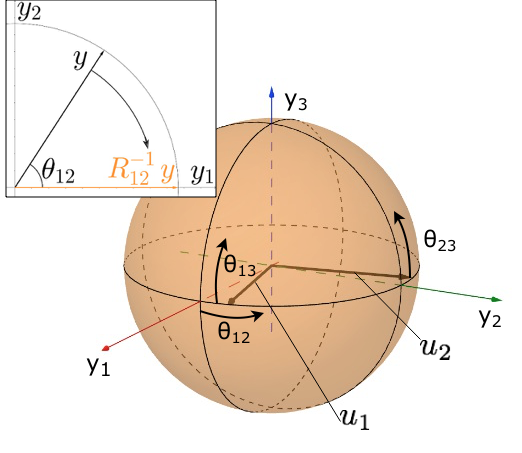
\includegraphics[width=0.4\textwidth]{figures/stiefel_geom_new.png}
\vspace{.05in}
\caption{(Inset) Givens rotations can be used to rotate a vector so as to eliminate its component in a certain direction. (Main Figure) A $p$-frame on the Stiefel manifold can be visualized as a set of rigidly connected orthogonal basis vectors, $u_1$ and $u_2$, shown here in black. One can move about the Stiefel manifold and describe any $p$-frame by simultaneously applying rotations matrices of a prescribed angle to these basis vectors. Applying the rotation matrix $R_{12}(\theta_{12})$ corresponds to rotating the two basis vectors toegher in the (1,2)-plane, which by our convention is the $(x,y)$-plane. Similarly, simultaneously apply $R_{13}(\theta_{13})$ corresponds to a rotation of the 2-frame in the $(1,3)$ or $(x,z)$-plane, while $R_{23}(\theta_{23})$ corresponds to rotating $u_2$ about $u_1$.}
\label{fig:StiefelGeom}
\end{figure}

\noindent In the Givens reduction algorithm, these rotation matrices are applied one-by-one to $A$ in this way to eliminate all elements below the diagonal. First, all elements in the first column below the first row are eliminated by successively applying the rotation matrices $R_{12}^{-1}(\theta_{12}), R_{13}^{-1}(\theta_{13}), \cdots, R_{1n}^{-1}(\theta_{1n})$  (Figure \ref{fig:givens_reduction}). Because multiplication by $R_{ij}(\theta_{ij})$ only affects elements $i$ and $j$ of a vector, once the $j$th element is zeroed out, the subsequent rotations, $R_{13}^{-1}(\theta_{13}), \cdots, R_{1n}^{-1}(\theta_{1n})$, will leave the initial changes unaffected. Similarly, once the first column of $A$ is zeroed out below the first element, the subsequent rotations, which do not involve the first element will leave the column unaffected. The rotations  $R_{23}^{-1}(\theta_{23}), \cdots, R_{2n}^{-1}(\theta_{2n})$ can thus be applied to zero out the second column, while leaving the first column unaffected. This results in the upper triangular matrix

\begin{figure}[h]
\centering
\vspace{.1in}
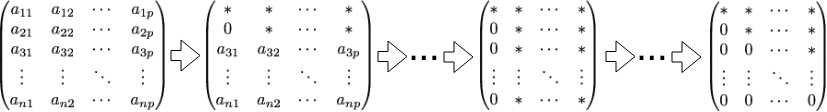
\includegraphics[width=1.0\textwidth]{figures/givens_reduction.png}
\vspace{.05in}
\caption{The Givens reduction eliminates lower diagonal elements of an $n \times p$ matrix one column at a time. Because each rotation, $R_{ij}(\theta_{ij})$, only affects rows $i$ and $j$, previously zeroed out elements do not change.}
\label{fig:givens_reduction}
\end{figure}

\begin{equation}
\label{eq:givens_reduction}
R_* := \underbrace{R_{pn}^{-1}(\theta_{pn}) \cdots R_{p,p+1}^{-1}(\theta_{p,p+1})  \cdots R_{2n}^{-1}(\theta_{2n}) \cdots R_{23}^{-1}(\theta_{23}) \cdots R_{1n}^{-1}(\theta_{1n}) \cdots R_{12}^{-1}(\theta_{12})}_{Q_*^{-1}} A.
\end{equation}

\noindent Crucially, the product of rotations, which we call $Q_*^{-1}$, is orthogonal since it is simply the product of rotation matrices which are themselves orthogonal. Thus its inverse can be applied to both sides of Equation \ref{eq:givens_reduction} to obtain

\begin{equation}
Q_* R_* = A.
\end{equation}

\noindent The familiar $QR$ form can be obtained by setting $Q$ equal to the first $p$ columns of $Q_*$ and setting $R$ equal to the first $p$ rows of $R_*$. The Givens reduction is summarized in Algorithm \ref{alg:givens_reduction}.

\begin{algorithm}[h]
\SetAlgoLined
\KwIn{$A$}
\KwResult{$Q,R$} 
 $Q_*^{-1} = I$
  $R_* = A$
 
 \For{$i$ in 1:p}{
 \For{$j$ in (i+1):n}{
    
    $\theta_{ij} = \arctan(Y[j,i]/Y[i,i])$
    
    $Q_*^{-1} = R_{ij}^{-1}(\theta_{ij}) Q_*^{-1}$
    
    $R_* = R_{ij}^{-1}(\theta_{ij}) R_*$

 }
 }
return $Q_*[,1:p], R_*[1:p,1:p]$
\\
\caption{Psuedo-code for the Givens reduction algorithm for obtaining the $QR$ factorization of a matrix $A$.}
 \label{alg:givens_reduction}
\end{algorithm}

%%%%%%%%%%%%%%%%%%%%%%%%%
\subsection{The Geometry of Orthogonal Matrices}\label{givens_stiefel_geometry}
%%%%%%%%%%%%%%%%%%%%%%%%%
The Stiefel manifold, $V_{p,n}$,  consists of $p$-frames: ordered sets of $p$ $n$-dimensional unit-length vectors, where $p \le n$. $p$-frames naturally correspond to $n \times p$ orthogonal matrices which can be used to define the Stiefel manifold succinctly as

\begin{equation}
V_{p,n} := \{Y \in \mathbb{R}^{n \times p}: Y^TY = I \}.
\end{equation}

\noindent Geometrically, an element of the Stiefel manifold can be pictured as a set of orthogonal, unit-length vectors that are rigidly connected to one another. A simple case is $V_{1,3}$, which consists of a single vector, $u_1$, on the unit sphere. This single vector can be represented by two polar coordinates that we naturally think of as longitude and latitude, but can also be thought of simply as subsequent rotations of the standard basis vector $e_1 := (1,0,0)^T$ in the $(x,y)$ and $(x,z)$ planes, which we refer to as the $(1,2)$ and $(1,3)$ planes for generality. In mathematical terms, $u_1$ can be represented as $u_1 = R_{12}(\theta_{12}) R_{13}(\theta_{13}) e_1$~(Figure \ref{fig:StiefelGeom}). 

\noindent Continuing without geometric interpretation, $V_{2,3}$ can be pictured as a vector in $V_{1,3}$ that has a second orthogonal vector, $u_2$, that is rigidly attached to it as it moves about the unit sphere. Because this second vector is constrained to be orthogonal to the first, its position can be described by a single rotation about the first vector. Thus elements of $V_{2,3}$ can be represented by three angles: two angles, $\theta_{12}$ and $\theta_{13}$, that represent how much to rotate the first vector, and a third angle, $\theta_{23}$ that controls how much the second vector is rotated about the first (Figure \ref{fig:StiefelGeom}). Mathematically this can be represented as the $3 \times 2$ orthogonal matrix $R_{12}(\theta_{12}) R_{13}(\theta_{13}) R_{23}(\theta_{23}) (e_1, e_2)$.

\noindent Although elements of the Stiefel manifold can be represented by $n \times p$ matrices, their inherent dimension is less than $np$ because of the constraints that the matrices must satisfy. The first column must satisfy a single constraint: the unit-length constraint. The second column must satisfy two constraints: not only must it be unit length, but it must also be orthogonal to the first column. The third column must additionally be orthogonal to the second column, giving it a total of three constraints. Continuing in this way reveals the inherent dimensionality of the Stiefel manifold to be

\begin{equation}
\label{eq:stiefel_dimension}
d := np - 1 - 2- \cdots p  = np - \frac{p(p+1)}{2}.
\end{equation}

%%%%%%%%%%%%%%%%%%%%%%%%%
\subsection{Obtaining the Givens Representation}\label{givens_representation_introduction}
%%%%%%%%%%%%%%%%%%%%%%%%%
The Givens reduction applied to an orthogonal matrix gives rise to a representation of the Stiefel manifold that generalizes the intuitive geometric interpretation described above. When applied to an $n \times p$ orthogonal matrix $Y$, the Givens reduction yields 

\begin{equation}
\label{eq:inverse_givens_representation}
R_{pn}^{-1}(\theta_{pn}) \cdots R_{p,p+1}^{-1}(\theta_{p,p+1})  \cdots R_{2n}^{-1}(\theta_{2n}) \cdots R_{23}^{-1}(\theta_{23}) \cdots R_{1n}^{-1}(\theta_{1n}) \cdots R_{12}^{-1}(\theta_{12}) Y = I_{n,p}
\end{equation}

\noindent where $I_{p,n}$ is defined to be the first $p$ columns of the $n \times n$ identity matrix, i.e. the matrix consisting of the first $p$ standard basis vectors $e_1, \cdots, e_p$. The first $n-1$ rotations transform the first column into $e_1$, since it zeros out all elements below the first and the orthogonal rotations do not affect the length of the vector which by hypothesis is unit length. Similarly, the next $n-2$ rotations will leave the length of the second column and its orthogonality to the first column intact because again, the rotation matrices are orthogonal. Because the second column must be zero below its second element it must be $e_2$. Continuing in this way explains the relationship in Equation \ref{eq:inverse_givens_representation}.

\noindent Because $Y$ was taken to be an arbitrary orthogonal matrix, then it is clear from Equation \ref{eq:inverse_givens_representation} that any orthogonal matrix $Y$ can be factored as

\begin{equation}
\label{eq:givens_representation}
Y = R_{12}(\theta_{12}) \cdots R_{1n}(\theta_{1n})  \cdots R_{23}(\theta_{23}) \cdots R_{2n}(\theta_{2n}) \cdots R_{p,p+1}(\theta_{p,p+1}) \cdots R_{pn}(\theta_{pn}) I_{n,p}.
\end{equation}

\noindent Defining $\Theta := (\theta_{12} \cdots \theta_{1n} \cdots \theta_{23} \cdots \theta_{2n} \theta_{p,p+1} \cdots \theta_{pn})$ we can consider any orthogonal matrix as a function, $Y(\Theta)$, of these angles, effectively parameterizing the Stiefel manifold and yielding the Givens representation. The Givens representation is a smooth representation with respect to the angles $\Theta$ \citep{shepard2015representation},  and lines up with our geometric insight discussed in the previous subsection.


%%%%%%%%%%%%%%%%%%%%%%%%%
%%%%%%%%%%%%%%%%%%%%%%%%%
%%%%%%%%%%%%%%%%%%%%%%%%%
\section{The Givens Representation for Bayesian Inference of Orthogonal Matrix Parameters} \label{implementation}
%%%%%%%%%%%%%%%%%%%%%%%%%
%%%%%%%%%%%%%%%%%%%%%%%%%
%%%%%%%%%%%%%%%%%%%%%%%%%

Practical use of the Givens representation in a general Bayesian inference framework involves solving several practical challenges. In addition to the standard change of measure term required in any transformation of a random variable, care must be taken to address certain pathological cases of the Givens representation that occur due to the different topologies of the Stiefel manifold and Euclidean space. We further describe these challenges and explain how we overcome them in practice. We also briefly remark on how the Givens representation can be leveraged in practice to solve issues with identifiability and define new and useful distributions over the Stiefel manifold. We conclude the section by describing how the computation of the Givens representation scales in theory, particularly in comparison to EMHMC.

%%%%%%%%%%%%%%%%%%%%%%%%%
\subsection{Transformation of Measure Under the Givens Representation}\label{measureGivens}
%%%%%%%%%%%%%%%%%%%%%%%%%
As is usual in any transformation of random variables, care must be taken to include a Jacobian determinant term in the transformed density to account for a change of measure under the transformation. For a posterior density over orthogonal matrices that takes the form $p_Y(Y)$, the proper density over the transformed random variable, $\Theta(Y)$, takes the form $p_\Theta(\theta) = p_{Y}(Y(\Theta)) |J_{Y(\Theta)}(\Theta)|$ \citep{keener2011theoretical}. Intuitively, this extra Jacobian determinant term accounts for how probability measures are distorted by the transformation (Figure \ref{fig:AreaForm}). Unfortunately, the Givens representation, $Y(\Theta)$, is map from a space of dimension $d := np - p(p+1)/2$ to a space of dimension $np$. Hence the determinant is non-square and thus undefined.

\begin{figure}[h]
\centering
\vspace{.1in}
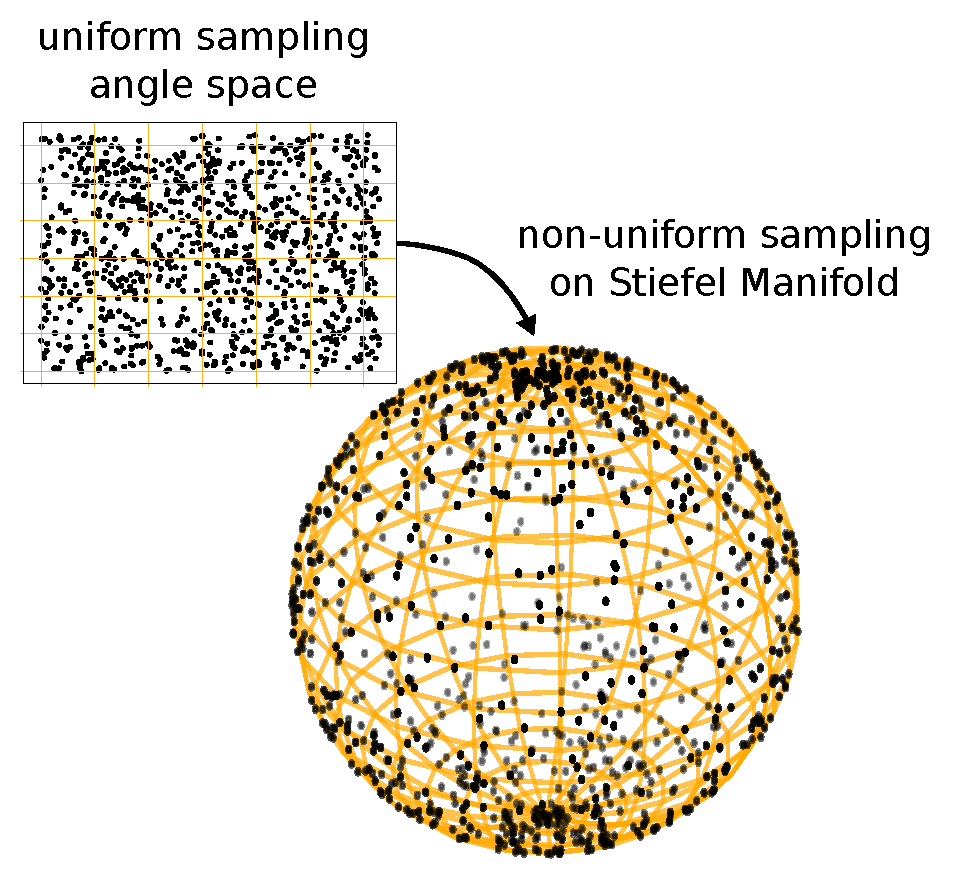
\includegraphics[width=0.5\textwidth]{figures/AreaForm_atz.pdf}
\vspace{.05in}
\caption{Uniform sampling in the Givens representation coordinates does not necessarily lead to uniform sampling over the Stiefel manifold without the proper measure adjustment term. Under the mapping, regions near the pole are shrunk to regions on the sphere with little area, as opposed to regions near to the equator which the transform maps to much larger areas on the sphere. Intuitively, the change-of-measure term quantifies this proportion of shrinkage in area.}
\label{fig:AreaForm}
\end{figure}


\noindent To compute the change of measure term analogous to the Jacobian determinant, one must appeal to the algebra of differential forms. Denote the product of $n \times n$ rotation matrices in the Givens representation by $G$, i.e. 


\begin{equation}
G := R_{12}(\theta_{12}) \cdots R_{1n}(\theta_{1n})  \cdots R_{23}(\theta_{23}) \cdots R_{pn}(\theta_{pn}) \cdots R_{p,p+1}(\theta_{p,p+1}) \cdots R_{pn}(\theta_{pn}),
\end{equation}

\noindent and denote its $j$th column by $G_j$. \cite{muirhead2009aspects} shows that the proper measure form for a signed surface element of $V_{p,n}$ is the differential form

\begin{equation}
\label{eq:WedgeForm}
\bigwedge_{i=1}^p \bigwedge_{j=i+1}^n G_j^T\, dY_i.
\end{equation}

\noindent Letting $J_{Y_i(\Theta)}(\Theta)$ be the Jacobian of the $i$th column of $Y$ with respect to the angle coordinates of the Givens representation, this differential form can be written in the coordinates of the Givens representation as

\begin{equation}
\label{eq:WedgeForm_givens}
\bigwedge_{i=1}^p \bigwedge_{j=i+1}^n G_j^T\, J_{Y_i(\Theta)}(\Theta) d\Theta.
\end{equation}

\noindent Because this is a wedge product of $d$ $d$-dimensional elements, Equation \ref{eq:WedgeForm_givens} can be conveniently written as the determinant of the $d \times d$ matrix

\begin{equation}
\label{eq:measure_matrix_form}
\begin{pmatrix}
G_{2:n}^T J_{Y_1(\Theta)}(\Theta)\\
G_{3:n}^T J_{Y_2(\Theta)}(\Theta)\\
\vdots\\
G_{p:n}^T J_{Y_p(\Theta)}(\Theta)
\end{pmatrix}
\end{equation}

\noindent where $G_{k:l}$ denote columns $k$ through $l$ of $G$. As we show in the appendix, this term can be analytically simplified to the following simple product whose absolute value serves as our measure adjustment term:

\begin{equation}
\label{eq:final_change_of_measure}
J_{Y(\Theta)}(\Theta) = \prod_{i=1}^p \prod_{j=i+1}^n \cos^{j-i-1} \theta_{ij}.
\end{equation}

%%%%% EXAMPLE FOR 3x1 CASE
%To build intuition we provide a simple example of using differential forms to compute an a change of measure factor. For a more thorough introduction to differential forms and their use in probability and statistics we refer the reader to the excellent tutorial by \cite{edelman200518} as well as the more thorough exposition of \cite{muirhead2009aspects}.

%Consider an element $Y \in V_{1,3}$ i.e. a vector on the unit sphere. The differential $dY$ of $Y$ is known as a one-form and can be visualized as an infinitessimal change in $Y$ that lies in the plane perpendicular to $Y$ known as the cotangent space. Defining $G := R_{12}(\theta_{12})R_{13}(\theta_{13}) I$, a basis for this cotangent space is formed by the second and third columns of $G$, $G_2$ and $G_3$.  This can be seen by observing that . Thus any arbitrary one-form can be represented in this basis by the coordinates $(G_2^T dY, G_3^T dY)$

%The Givens representation $Y(\Theta) = R_{12}(\theta_{12})R_{13}(\theta_{13})e_1$ can be thought of as mapping points in the grid formed by $\theta_{12}$ and $\theta_{13}$ to a points on the sphere. Just as points in this space can be mapped by the transformation onto points on the sphere so to can one-forms, be mapped to one-forms on the sphere (Figure). In fact, the columns of the Jacobian, $J_{Y(\Theta)(\Theta)}$ are the precise one-forms that the one-forms $d\theta_{12}$ and $d\theta_{13}$ get mapped to by the transformation. Similarly, the the transformation can be thought of as mapping the two-dimensional parallelogram formed by $d\theta_{12}$ and $d\theta_{13}$, otherwise known as a two-form, to the two-form formed by the columns of $J_{Y(\Theta)(\Theta)}$. The area of this latter parallelogram is precisely the change of measure term we seek. It can be obtained by first projecting these three-dimensional one-forms down to a two-dimensional parallel plane. Once projected, the two-dimensional representation can be used to form a $2 \times 2$ matrix whose determinant represents the area formed by the parallelogram. If we define $G:=  R_{12}(\theta_{12})R_{13}(\theta_{13})$, then this parallel plane is simply 


%\begin{algorithm}[h]
%\SetAlgoLined
%\KwIn{Matrix $G$ from Equation \ref{eq:Gmatrix}. Jacobian matrices $J_{Y_i}(\Theta)$, $i = 1,\cdots, p$.}
%\KwResult{Measure adjustment factor for the Givens Representation.} 
%$d = np - p(p+1)/2$

%$AreaMatrix = Identity(d)$
 
%$idx = 0$
 
 %\For{$i$ in 0:p}{
 
% 	$OneForms = (G[(i+1):n,]^T J_{Y_i}(\Theta))^T$
    	
%	 \For{$j$ in 0:n}{
%	 	$AreaMatrix[,idx] = OneForms[,j]$
		
%		$idx = idx + 1$
%	 }

% }
%$S = log(det(AreaMatrix))$
%\\
%\caption{Psuedo-code for obtaining the measure adjustment factor for the Givens Representation.}
% \label{alg:diff_form}
%\end{algorithm}

%%%%%%%%%%%%%%%%%%%%%%%%%
\subsection{Implementation of Angle Coordinates}
%%%%%%%%%%%%%%%%%%%%%%%%%
When using the Givens representation for general Bayesian inference in practice, care must be taken to properly account for pathologies that arise when mapping the Stiefel manifold to Euclidean space. We let $\theta_{12}, \theta_{23}, \cdots \theta_{p,p+1}$ range from $-\pi$ to $\pi$ and we refer to these specific coordinates as the latitudinal coordinates to evoke the analogy for the simple spherical case. Similarly, we let the remaining coordinates range from $-\pi/2$ to $\pi/2$ and we refer to these coordinates as longitudinal coordinates. This choice of intervals defines a coordinate chart from Euclidean space to the Stiefel manifold, i.e. a mapping between the two spaces. Because the topology of these two space differ, certain connectedness properties of the Stiefel manifold can not be accurately represented in the Givens representation. For example, when representing $V_{1,3}$ in Euclidean space using the Givens representation, contiguous regions of the manifold on either side of the sliver corresponding to $\theta_{12} = \pi$ are disconnected (Figure \ref{fig:pathologies}). As we show, this can lead to misleading results when applying sampling methods such as HMC to sample densities over the Stiefel manifold using the Givens representation. In addition to these disconnected regions, the coordinate chart will also contain singularities where the adjustment term (Equation \ref{eq:final_change_of_measure}) approaches zero forcing the transformed density to equal zero at a point where there might be positive density. On the sphere, this happens at the North and South poles where the longitudinal coordinates become exactly $-\pi/2$ or $\pi/2$ (Figure \ref{fig:pathologies}). As we discuss, this can cause numerical issues for algorithms like HMC. To overcome the first issue, we introduce an auxiliary parameter for each latitudinal angle that connects the regions that are otherwise disconnected in the coordinates of the Givens representation. To overcome the second issue, we block off a small region of the Stiefel manifold near the pole and justify this choice using theoretical arguments and numerical experiments.

\begin{figure}[h]
\centering
\vspace{.1in}
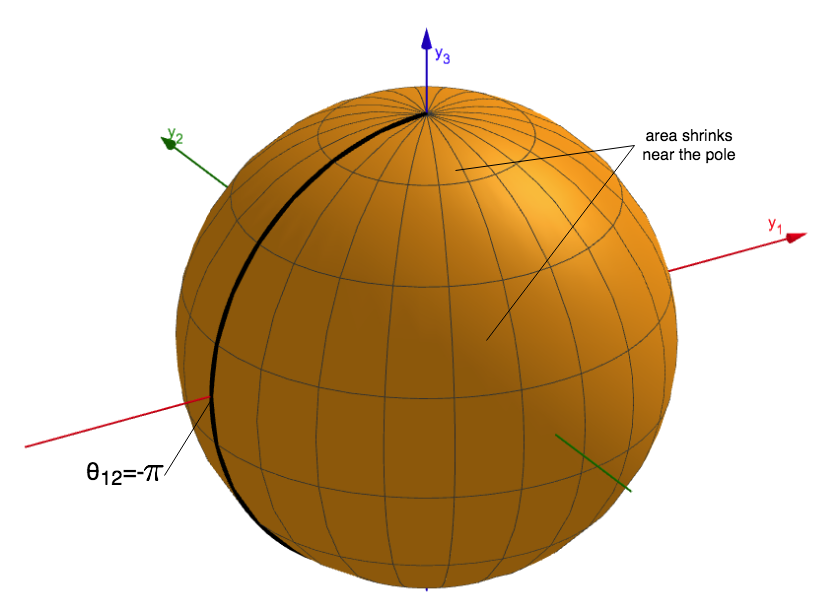
\includegraphics[width=0.5\textwidth]{figures/sliver_globe.png}
\vspace{.05in}
\caption{The angular coordinate chart has an infinitesimal sliver of measure zero lying at $\theta_{12} = -\pi = \pi$ that separates two otherwise connected parts of the sphere. Trajectories, $Y(t)$, over the Stiefel manifold that cross this sliver have no equivalent representation, $\Theta(t)$ in the coordinates of the Givens representation. This can become particularly problematic when there is significant probability mass on both sides of the sliver. The grid over the sphere reveals how the Givens representation maps areas that are the same size in the $\Theta$ coordinates to smaller and smaller regions on the sphere the closer they are to the poles. Thus the measure adjustment term (Equation \ref{eq:final_change_of_measure}), which measures how the transform changes the area of these infinitesimal regions goes to zero near the poles, making the equivalent density at these points zero.}
\label{fig:pathologies}
\end{figure}

%%%%%%%%%%%%%%%%%%%%%%%%%
\subsubsection{Introducing Auxiliary Parameters}
%%%%%%%%%%%%%%%%%%%%%%%%%
\noindent As is routinely done in practice, a logistic transform can be used to map the interval $[-\pi,\pi]$ to the unconstrained interval $(-\infty, \infty)$. Unfortunately, this leaves regions of parameter space that should otherwise be connected, disconnected by the aforementioned set of measure zero. For a distribution over the Stiefel manifold that is not sufficiently concentrated away from this measure-zero-set, this can lead to samples that are representative of only one of the regions on either side of the sliver (Figure \ref{fig:donut}, upper).

\begin{figure}[h]
\centering
\vspace{.1in}
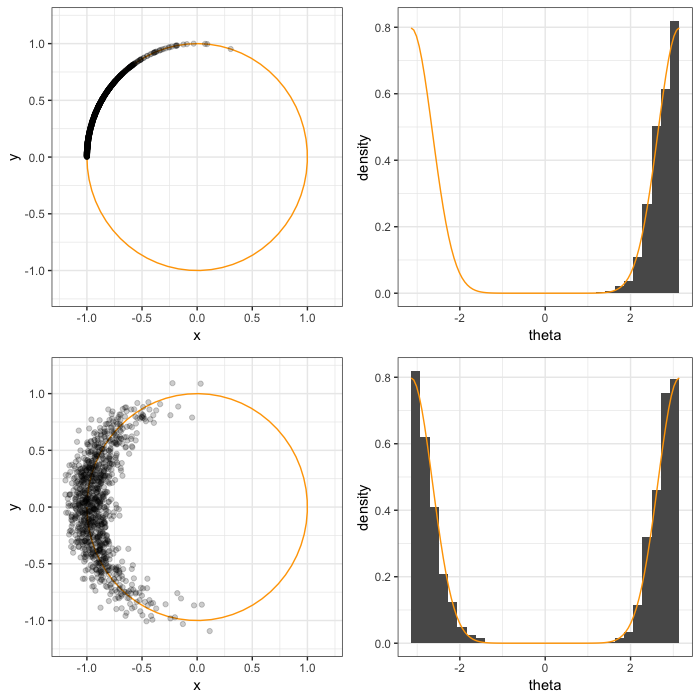
\includegraphics[width=0.6\textwidth]{figures/donut.png}
\vspace{.05in}
\caption{(Upper) 1000 samples from a Von Mises distribution with parameters $\mu = -\pi$ and $\kappa = 5$ sampled over the space $\theta \in [-\pi, \pi]$ using Stan. Most of the mass of the distribution is concentrated at the ends of the interval while little mass is concentrated towards the middle. Because these two ends of the interval are disconnected in this representation, the sampler gets ``stuck" in the left-most mode. (Lower) 1000 samples from the equivalent distribution sampled over the $(x,y)$-space. By introducing an auxiliary coordinate, one can effectively replicate the topology of a circle, effectively ``wrapping" the two ends of the interval so that the sampler avoids getting stuck in one region.}
\label{fig:donut}
\end{figure}

\noindent To handle this multimodality introduced by reparameterizing in terms of Givens angles, we introduce for each angle parameter, $\theta_{ij}$, an independent auxiliary parameter, $r_{ij}$. We then transform the density to sample over $x_{ij} = r_{ij} \cos \theta_{ij}$ and $y_{ij} = r_{ij} \sin \theta_{ij}$. In the transformed space the two ends of the interval are connected, producing samples that are distributed more evenly across the two disconnected regions (Figure \ref{fig:donut}, lower). Formally, we assign to $r$ a marginal distribution with density $p_r(r)$ so that $\theta$ and $r$ are independent and the distribution of $\theta$ is left untouched by the introduction of the auxiliary parameter. This provides the joint density $p_{\theta, r}(\theta, r) = p_\theta(\theta) p_r(r)$ which we then transform to the equivalent density over the unconstrained $(x,y)$-space by the simple change-of-variables formula between two-dimensional polar coordinates and two-dimensional Euclidean coordinates:

\begin{eqnarray}
p_{x, y}(x,y) &=& p_{\theta, r}(\mathrm{arctan} \left(y/x), \sqrt{x^2 + y^2} \right) \frac{1}{r}.
\end{eqnarray}

\noindent This again leaves the distribution of $\theta$ unaffected, however, in the new space, paths $\theta(t)$ that cross the region of parameter space at $\theta = \pi$ can actually be represented. In practice, we set  $p_r(r)$ to a normal density with mean one and standard deviation 0.1. Although $r_{ij}$ does not necessarily need to be set to this particular distribution to achieve the correct marginal distribution over $\theta$, this choice helps avoid the region of parameter space $r = 1$ and the transformed density is ill-defined.

%%%%%%%%%%%%%%%%%%%%%%%%%
\subsubsection{Truncating Parameter Space Near Singularities}
%%%%%%%%%%%%%%%%%%%%%%%%%
\noindent  Even with the usual change of variables formula and the measure adjustment term (Equation \ref{eq:final_change_of_measure}), a finite density function over the Stiefel manifold specified in terms of the canonical coordinates, will not be completely equivalent to the transformed density over the Stiefel manifold. In particular, when any of the longitudinal angles has absolute value equal to $\pi/2$, Equation \ref{eq:final_change_of_measure} will equal zero. Thus the transformed density will be zero on this set of measure zero even when the original density is non-zero on that set. Because of finite numerical precision, in practice this creates a region of the Stiefel manifold that can not be sampled numerically despite having positive a positive probability mass. This effectively reduces the space being sampled by limiting all longitudinal angles to the region $[-\pi/2 + \epsilon, \pi/2 - \epsilon]$. Despite this concern, as we show both theoretically and experimentally, the exceedingly small volume of this region justifies the use of the Givens representation in practice.

%\begin{equation}
%\log |J_{Y(\Theta)}(\Theta)| = \sum_{i=1}^p \sum_{j=i+1}^n (j-i-1) \log |\cos \theta_{ij}|.
%\end{equation}

%\noindent and its partial derivatives

%\begin{equation}
%\frac{\partial}{\partial \theta_{ij}}\log |J_{Y(\Theta)}(\Theta)| = -(j-i-1) |\tan \theta_{ij}|.
%\end{equation}

%\noindent For both expressions, the terms involving the latitudinal coordinates drops out leaving expression that are only in terms of the longitudinal coordinates which take on values between $\pi/2$ and $\pi/2$. However, the partial derivatives grow unbounded as $\theta_{ij}$ approaches either of these endpoints. When sampling near these points this unbounded gradient can cause numerical issues for HMC such as divergences. Alternatively, the difficulty of sampling near these regions can force automatic warmup routines for HMC to select an unreasonably small and inefficient step size to in an effort to maintain high average accept rates. Luckily, on the logit scale, gradients of the resulting transformed density are finite even at $|\theta_{ij}| = \pi/2$. In particular, .

%\noindent Consider the Givens representation $[-\pi/2 + \epsilon, \pi/2 - \epsilon]$ where $\epsilon$ is a small value (on the order of $10^{-5}$ in our experiments), rather than the full interval $[-\pi/2, \pi/2]$. This change effectively blocks off a small portion of parameter space surrounding the singularities of the change of measure term. In the spherical case, this is equivalent to two small patches at each pole that is blocked off. While this restricts part of parameter space, we show theoretically and empirically, that for a modestly small $\epsilon$, the bias incurred becomes negligible. 

\noindent We show that for general $n$ and $p$, the volume of this blocked off region is $\mathcal{O}(p \epsilon^2)$. First, the uniform density over $V_{pn}$ in the Givens representation is simply a constant times Equation \ref{eq:final_change_of_measure}. However, since this density factors in to a product of independent terms, the probability that at least one longitudinal angle falls within the $\epsilon$ region is simply the sum of the individual probability of each angles falling within the region. Each of these individual probabilities is proportional to $\cos^{j-i-1} \theta_{ij}$, which for small $\epsilon$ can be bounded by $\epsilon^{j-i-1}$ over the interval $[\pi/2 - \epsilon, \pi/2]$. Thus the probability of falling within the $\epsilon$ region is bounded by a constant times the following quantity:

\begin{equation}
\label{eq:bound_on_epsilon_vol}
\sum_{i=1}^p \sum_{j=i+2}^n 2 \int_{\pi/2-\epsilon}^{\pi/2} \epsilon^{j-i-1} d\theta_{ij} = \sum_{i=1}^p \sum_{j=i+2}^n 2 \epsilon^{j-i} = \sum_{i=1}^p \mathcal{O}(\epsilon^2) = \mathcal{O}(p \epsilon^2).
\end{equation}

\noindent Because this quantity falls off with the square of $\epsilon$, even for modestly small $\epsilon$, the probability of a uniformly sampled point falling within the $\epsilon$ region is small. Empirical results further illustrate this. For various values of $n, p,$ and $\epsilon$ we drew 100,000 samples uniformly form the Stiefel manifold by sampling the elements of an $n \times p$ matrix from a standard normal distribution, then taking the QR factorization of this matrix, a common technique for uniformly sampling the Stiefel manifold \citep{muirhead2009aspects}. We then took these samples, converted them in to their Givens representation, and calculated the number of samples that had any longitudinal angle within the region $[-\pi/2, -\pi/2+\epsilon]$ or the region $[\pi/2-\epsilon, \pi/2]$. The results are closely explained byEquation \ref{eq:bound_on_epsilon_vol}. In particular, the proportion of samples that fell within this region does not change much for fixed $p$ and increasing $n$, the proportion increases linearly with $p$, and it decreases quadratically with $\epsilon$ (Table \ref{tab:uniform_epsilon_region}).  

\begin{table*}
\begin{tabular}{|cc||ccccc|}
\hline
$p$ & $n$  & $\epsilon = 0.1$ & $\epsilon = 0.05$ & $\epsilon = 0.025$ & $\epsilon = 0.0125$ & $\epsilon = 1e-5$\\
\hline
\hline
1 & 10 & 490 & 114 & 22 & 4 & 0\\
1 & 20 & 499 & 118 & 25 & 4 & 0\\
1 & 50 & 570 & 148 & 32 & 6 & 0 \\
\hline
3 & 10 & 1,612 & 381 & 79  & 15 & 0\\
3 & 20 & 1,665 & 398 & 78 & 19 & 0\\
3 & 50 & 1,712 & 416 & 100  & 24 & 0\\
\hline
10 & 10 & 4,260 & 1,071 & 258 & 59 & 0\\
10 & 20 & 5,342 & 1,336 & 357 & 91 & 0\\
10 & 50 & 5,266 & 1,368 & 334 & 90 & 0 \\
\hline
\end{tabular}
\caption{The number of uniform samples out of 100,000 that fell within the $\epsilon$ region for various values of $n, p,$ and $\epsilon$. Samples are taken uniformly from the Stiefel manifold using the QR factorization method. As the theoretical bound suggests, the number of samples falling in this region increases negligibly for fixed $p$ and increasing $n$, it increases linearly with $p$, and it decreases quadratically as $\epsilon$ decreases. In particular, whenever $\epsilon$ is halved, the number of sample falling within the region decrease by about a fourth. We also note that for $\epsilon = 1e-5$, the value we used for most of our experiments, the number of samples falling within the $\epsilon$ region is zero for all settings.}
\label{tab:uniform_epsilon_region}
\end{table*}

\noindent For non-uniform distributions with a probability density $p(\Theta)$ that is finite in the $\epsilon$ region, the probability of any of the longitudinal angles falling within the $\epsilon$ region can again be bounded by a constant times $\mathcal{O}(p \epsilon^2)$. We took 100,000 samples from the von Mises Fisher distribution over $V_{1,3}$ with parameters $\mu = (0,0,1)$ and $\kappa = 1, 10, 100$, and 1000 using the simulation method of \citet{wood1994simulation} as implemented in the R package Rfast. For fixed $\kappa$ the probability of a sample falling in the $\epsilon$ region drops off with the square of $\epsilon$ as the bound would suggest. This holds true even when probability mass is highly concentrated near these regions (Table \ref{tab:vmf_epsilon_region}).  

\begin{table*}
\begin{tabular}{|c||ccccc|}
\hline
$\kappa$  & $\epsilon = 0.1$ & $\epsilon = 0.05$ & $\epsilon = 0.025$ & $\epsilon = 0.0125$ & $\epsilon = 1e-5$\\
\hline
\hline
1 & 630 & 163 & 38 & 9 & 0\\
10 & 4,839 & 1,220 & 317 & 81 & 0\\
100 & 39,287 & 11,658 & 3,086 & 764 & 0 \\
1,000  & 99,295 & 71,066 & 26,643 & 7,473 & 0 \\
\hline
\end{tabular}
\caption{The number of samples from a von Mises Fisher distribution with $\mu = (0,0,1)$ and $\kappa = 1, 10, 100$ and 1000 that fell within the $\epsilon$ region for various values of $n, p,$ and $\epsilon$. For each value of $\kappa$ 100,000 total samples were taken. As the theoretical bound suggests, the number of samples that fill within the $\epsilon$ region fall with the square of $\epsilon$ so that even for a modestly small value of $\epsilon = 1e-5$, none of the 100,000 samples fall within this region even in the highly concentrated case ($\kappa = 1,000$).}
\label{tab:vmf_epsilon_region}
\end{table*}

\noindent Because the probability of samples falling within the $\epsilon$ falls with the square of $\epsilon$, even for modestly small $\epsilon$, the distribution of derived quantities of $Y(\Theta)$ remains largely unaffected when sampling using the Givens representation with small enough $\epsilon$. We sampled the von Mises Fisher distribution with the same values of $\kappa$ using the Givens representation in Stan with an $\epsilon = 0.1, 0.05, 0.025, 0.0125,$ and $1e-5$. We then examined histograms and expectations of the principal angle $\arccos (\mu^T Y)$ which represents the angle between the sample and the direction at the pole lying directly in the middle of the $\epsilon$ region. For large $\epsilon$ and large $\kappa$ the bias induced by the $\epsilon$ region is evident when compared to samples using the method of \citet{wood1994simulation} since the sample can not get close enough to $\mu$. However, for any fixed $\kappa$ as $\epsilon$ is decreased, the bias decreases rapidly as the bound would suggest (Figure \ref{fig:epsilon_histogram}). Table \ref{tab:vmf_epsilon_region_expectations} illustrates this effect numerically using the expectation of the principal angle and the expectation of its square.

\begin{figure}[h]
\centering
\vspace{.1in}
\includegraphics[width=0.65\textwidth]{figures/epsilon_histogram.png}
\vspace{.05in}
\caption{Histograms of the principal angle, $\arccos (\mu^T Y)$, sampled under the von Mises Fisher distribution with $\mu = (0,0,1)$ and $\kappa = 1, 10, 100$ and 1000 using the Givens representation in Stan with various sizes of the $\epsilon$ area and using the method of \citet{wood1994simulation}. For small $\epsilon$ and large $\kappa$, the bias in the samples taken using the latter method is evident in the histograms. In particular, despite the large amount of mass near zero, the samples are never higher than a bound higher than zero that is dictated by $\epsilon$. As $\epsilon$ decreases, the bound rapidly becomes negligible because of the quadratic relationship between $\epsilon$ and the volume of the $\epsilon$ area. Thus for $\epsilon = 1e-5$, the histograms of the Givens representation method and the \citet{wood1994simulation} method become indistinguishable.}
\label{fig:epsilon_histogram}
\end{figure}

\begin{table*}
\begin{tabular}{|c||ccccc|c|}
\hline
 &   Givens &  &  &  & & Wood\\
\hline
$\kappa$ & $\epsilon = 0.1$ & $\epsilon = 0.05$ & $\epsilon = 0.025$ & $\epsilon = 0.0125$ & $\epsilon = 1e-5$ & \\
\hline
\hline
1 & 1.2027 & 1.2042 & 1.2008 & 1.1995 & 1.1986 & 1.2012\\
10 & 0.4181 & 0.4065 & 0.4031 & 0.4012 & 0.4019 & 0.4015\\
100 & 0.1657 & 0.1377 & 0.1290 & 0.1258 & 0.1261 & 0.1255 \\
1,000 & 0.1092 & 0.0657 & 0.0483 & 0.0422 & 0.0396 & 0.0398\\
\hline
\end{tabular}
\caption{The empirical expectation of the principal angle, $\arccos (\mu^T Y)$, sampled under the von Mises Fisher distribution with $\mu = (0,0,1)$ and $\kappa = 1, 10, 100$ and 1000 using the Givens representation in Stan with various sizes of the $\epsilon$ area and using the method of \citet{wood1994simulation}. As $\epsilon$ decreases, the empirical expectation computed using the Givens representation become much closer to those taken via the method of \citet{wood1994simulation}. For small $\kappa$ the expectations do not differ much even for large $\epsilon$ because much less mass concentrates near the $\epsilon$ regions.}
\label{tab:vmf_epsilon_region_expectations}
\end{table*}

%%%%%%%%%%%%%%%%%%%%%%%%%
%\subsection{Coordinate Charts and Identifiability}\label{charts_identifiability}
%%%%%%%%%%%%%%%%%%%%%%%%%
%For certain applications such as PPCA, it may be desirable to further limit parameter space to avoid symmetries that lead to identifiability issues in the posterior. In the Givens representation coordinates this is simply a matter of constraining the range of the longitudinal angles to the interval $[-\pi/2,\pi/2]$ (Figure \ref{fig:limiting_pca}). Unfortunately, as in the case of the full interval, this can lead to biased sampling due to regions of low mass separating regions of high mass in parameter space. However, this issue can be resolved by carefully connecting these regions via a simple mirroring technique which we describe.

%\begin{figure}[h]
%\centering
%\vspace{.1in}
%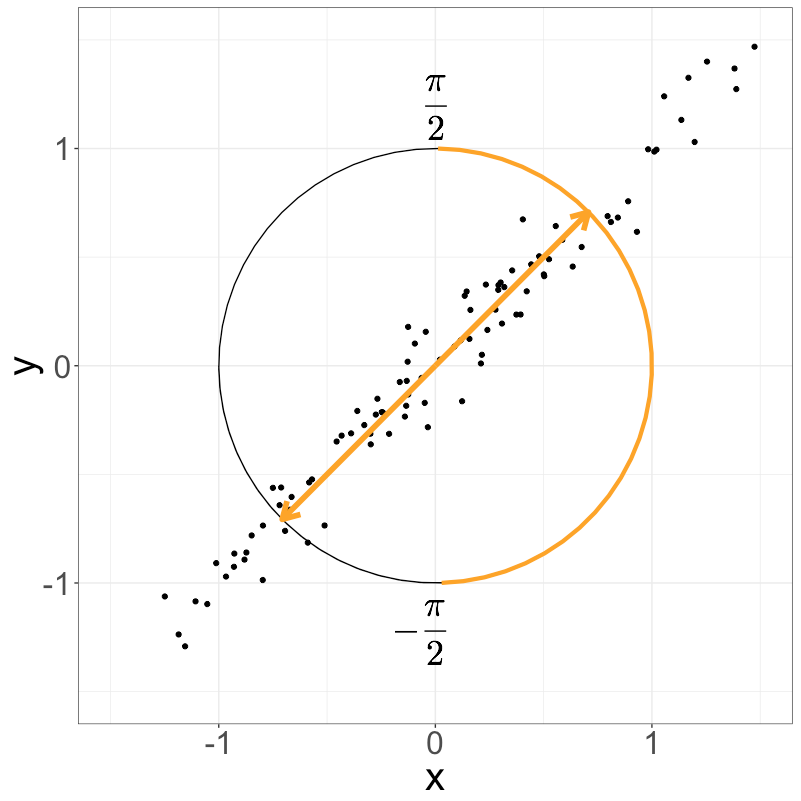
\includegraphics[width=0.4\textwidth]{figures/limiting_pca.png}
%\vspace{.05in}
%\caption{PPCA seeks to find the best lower dimensional $p$-frame to describe a high-dimensional set of points. For $n = 2$ and $p=1$, this corresponds to the vector that most closely describes a set of two-dimensional points that lie close to flat line. Since a $p$-frame and its negative can describe the data equally well, a multi-modal posterior over the Stiefel manifold results. By limiting the longitudinal angle to lie in the interval $[-\pi/2, \pi/2]$ the sampler does not consider this redundant mode.}
%\label{fig:limiting_pca}
%\end{figure}

%\noindent We can allow the original longitudinal and latitudinal coordinates, $\theta_\mathrm{lon}$ and $\theta_\mathrm{lat}$ to freely roam the Stiefel manifold using the aforementioned approach then define the new transformed parameters $\theta_\mathrm{lon}^*$ and $\theta_\mathrm{lat}^*$ to essentially be mirrored versions of these original coordinates. Specifically, we can define

%\begin{equation}
%\theta_\mathrm{lon}^*
%=
%\begin{cases}
%\theta_\mathrm{lon},& |\theta_\mathrm{lon}| \le \frac{\pi}{2}\\
%-\frac{\pi}{2}+(\theta_\mathrm{lon}-\frac{\pi}{2}),& \theta_\mathrm{lon} > \frac{\pi}{2}\\
%\frac{\pi}{2}+(\theta_\mathrm{lon}+\frac{\pi}{2}),& \theta_\mathrm{lon} < -\frac{\pi}{2}
%\end{cases}
%\end{equation}

%and

%\begin{equation}
%\theta_\mathrm{lat}^*
%=
%\begin{cases}
%\theta_\mathrm{lat},& |\theta_\mathrm{lon}| \le \frac{\pi}{2}\\
%-\theta_\mathrm{lat},& |\theta_\mathrm{lon}| > \frac{\pi}{2}.
%\end{cases}
%\end{equation}

%\noindent These transformed coordinates essentially mirror and reflect the original coordinates so that once the hemisphere is crossed, the path taken continues on the opposite side of the Stiefel manifold where there would naturally be an area of high posterior mass (Figure \ref{fig:givens_mirroring}). In fact, one can check that the PPCA likelihood (Equation \ref{eq:ppca_likelihood}) is continuous with respect to these new coordinates, allowing for efficient sampling even when there is appreciable posterior mass near the edge of the hemisphere.

%\begin{figure}[h]
%\centering
%\vspace{.1in}
%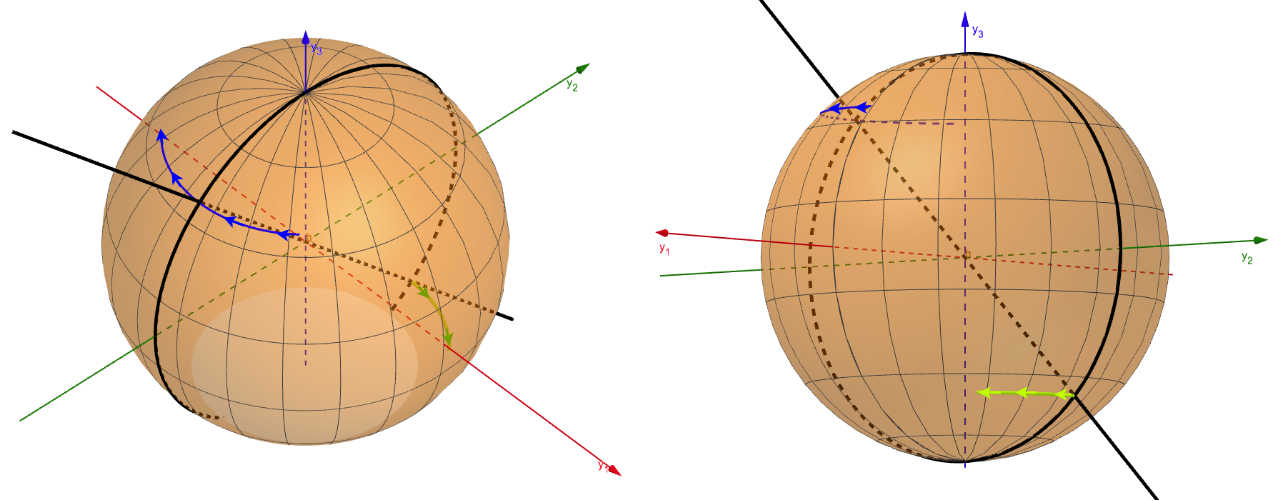
\includegraphics[width=0.9\textwidth]{figures/givens_mirroring.png}
%\vspace{.05in}
%\caption{Occasionally, the direction that best describes a high-dimensional dataset in PPCA (black line) is near the boundary of the longitudinal coordinate (thick black border). In this case, its negative will have an appreciable probability mass near it and the same density. Because of this continuity in the density, these areas of parameter space can be smoothly connected. Specifically, once the border is crossed (blue path) the coordinates now describe a point on the opposite end of the Stiefel manifold (green path).}
%\label{fig:givens_mirroring}
%\end{figure}

%%%%%%%%%%%%%%%%%%%%%%%%%
\subsection{New Distributions Using the Givens Representation}
%%%%%%%%%%%%%%%%%%%%%%%%%
Rather than placing priors over standard orthogonal matrix coordinates, $Y$, one can place priors over the coordinates of the Givens representation $\Theta$. In practice this leads to new classes of possible distributions. \noindent \cite{cron2016models} utilize sparsity promoting priors over the coordinates of the Givens representation to produce a distribution over the Stiefel manifold that favors sparse matrices. They apply this distribution to the estimation of normal mixture classification probabilities. \cite{leon2006statistical} make use of a different parameterization of orthogonal matrices to define a distribution over orthogonal matrices.

%\noindent  Distributions in terms Givens representation coordinates also have the added benefit of avoiding calculation of expensive orthogonal matrix densities such as the von Mises-Fisher matrix distribution. In particular, the density for the von Mises-Fisher matrix distribution takes the form $a(F) \exp(\mathrm{tr}\, Y^T F)$, where $a(F)$ is a normalizing constant involving an infinite sum \citep{khatri1977mises}.  For fixed priors over the Stiefel manifold, where $F$ is held constant, the normalizing term can be dropped from the unnormalized posterior for the purposes of inference (see e.g. \cite{hoff2009simulation}). However, if $F$ is an unknown being estimated, as is the case in say a multi-level model, then the normalizing term must be included in calculations involving the posterior, thus precluding use of the von Mises-Fisher matrix distribution in multi-level models. In contrast, multi-level modeling of orthogonal matrices can be straightforward in the Givens representation coordinates as we illustrate in Section \ref{coag}.

%%%%%%%%%%%%%%%%%%%%%%%%%
\subsection{Computational Scaling of the Givens Representation}\label{scaling}
%%%%%%%%%%%%%%%%%%%%%%%%%
The primary computational cost in using the Givens representation, is the series of $d$ $n \times n$ matrix multiplications applied to $I_{n,p}$ in 
Equation \ref{eq:givens_representation}. Fortunately, unlike dense matrix multiplication, applying a Givens rotation to an $n \times p$ matrix only involves two vector additions of size $p$ (Algorithm \ref{alg:givens}). Thus since $d$ scales on the order of $np$, computation of the Givens representation in aggregate scales as $\mathcal{O}(np^2)$.

\begin{algorithm}[h]
\SetAlgoLined
\KwIn{$\theta$}
\KwResult{$Y$} 
$Y = I_{n,p}$;
 idx = $d$
 
 \For{$i$ in p:1}{
 \For{$j$ in n:(i+1)}{
    
    $Y_i = \cos(\theta_{\mathrm{idx}}) Y[i,] - \sin(\theta_{\mathrm{idx}}) Y[j,]$
    
     $Y_j = \sin(\theta_{\mathrm{idx}}) Y[i,] + \cos(\theta_{\mathrm{idx}}) Y[j,]$
        
    $Y[i,] = Y_i$
    
    $Y[j,] = Y_j$
    
    $idx = idx - 1$
    
    log density += $(j-i-1) \log \cos \theta_{\mathrm{idx}}$
 }
 }
return $Y$
\\
\caption{Psuedo-code for obtaining the orthogonal matrix $Y$ from the Givens Representation as well as appropriately adjusting the log of the posterior density.}
 \label{alg:givens}
\end{algorithm}

\noindent In comparison, EMHMC involves an orthogonalization of an $n \times p$ matrix which scales as $\mathcal{O}(np^2)$ and a matrix exponential computation that scales as $\mathcal{O}(p^3)$. In practice, we find that EMHMC scales better when $p$ is much smaller than $n$, whereas the Givens representation scales better when $p$ is large and closer to $n$. We present benchmarks in Section \ref{scaling}.

%%%%%%%%%%%%%%%%%%%%%%%%%
%%%%%%%%%%%%%%%%%%%%%%%%%
%%%%%%%%%%%%%%%%%%%%%%%%%
\section{Results and Examples} \label{examples}
%%%%%%%%%%%%%%%%%%%%%%%%%
%%%%%%%%%%%%%%%%%%%%%%%%%
%%%%%%%%%%%%%%%%%%%%%%%%%

We demonstrate the use of the Givens representation and compare it with EMHMC for three common statistical examples from the literature. All Givens representation experiments were conducted in Stan using Stan's automatic warm-up and tuning options. For all Stan experiments we ensured that there were no divergences during post-warmup sampling and that all $\hat{R}$ were $1.01$ or below. All timing experiments were conducted on a 2016 Macbook Pro.


%%%%%%%%%%%%%%%%%%%%%%%%%
\subsection{Uniform Sampling on the Stiefel Manifold} \label{scaling_examples}
%%%%%%%%%%%%%%%%%%%%%%%%%
We sample uniformly from the Stiefel manifold of various sizes to assess the practical scalability of the Givens representation. We compare its sampling efficiency and $\hat{R}$ values to EMHMC on 500 post-warmup samples from each method (Table \ref{tab:rhat_neff}).  

\begin{table*}
\begin{tabular}{|cc||cc|cc|}
\hline
& & EMHMC & & Givens &\\
\hline
$p$ & $n$  & $\hat{R}$ & $n_{\mathrm{eff}}$ & $\hat{R}$ & $n_{\mathrm{eff}}$\\
\hline
\hline
1 & 10 & 1.00 & 231 & 1.00 & 496\\
1 & 100 & 1.00 & 317 & 1.00 & 488\\
1 & 1000 & 1.00 & 238 & 1.00 & 487 \\
\hline
10 & 10 & 1.00 & 408 & 1.00  & 390\\
10 & 100 & 1.00 & 473 & 1.00 & 487\\
10 & 1000 & 1.00 & 454 & 1.00  & 488 \\
\hline
100 & 100 & 1.00 & 484 & 1.00 & 479 \\
\hline
\end{tabular}
\caption{$\hat{R}$ and $n_{\mathrm{eff}}$ values averaged over all elements of the matrix parameter $Y$. }
\label{tab:rhat_neff}
\end{table*}

\noindent As mentioned in section \ref{measureGivens}, to uniformly samples the Stiefel manifold in the Givens representations, the change of measure term, Equation \ref{eq:final_change_of_measure}, must be computed as part of the likelihood. Meanwhile, uniform sampling over the Stiefel manifold is achieved in EMHMC simply using a constant likelihood because the method uses the original matrix coordinates. However, as mentioned in section \ref{scaling}, this comes at the cost of an expensive HMC update to ensure the updated parameter still satisfies the constraints.. In practice, we find that EMHMC scales better as $n$ is increased, although the approach using the Givens representation in Stan remains competitive (Figure \ref{fig:scaling}).

\begin{figure}[h]
\centering
\vspace{.1in}
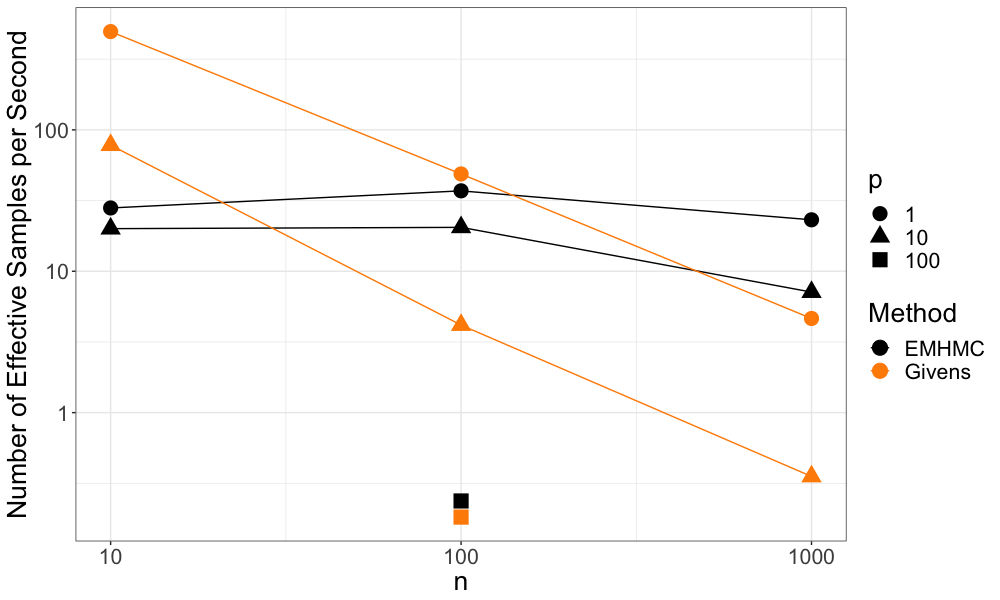
\includegraphics[width=0.8\textwidth]{figures/scaling.png}
\vspace{.05in}
\caption{For small values of $n$ the Givens representation approach in Stan produces more effective samplers per second while for larger values the EMHMC scales better since the primary cost of the matrix exponential remains constant.}
\label{fig:scaling}
\end{figure}

%%%%%%%%%%%%%%%%%%%%%%%%%
\subsection{Probabilistic PCA (PPCA)}
%%%%%%%%%%%%%%%%%%%%%%%%%
Factor Analysis (FA) and Probabilistic PCA (PPCA) \citep{tipping1999probabilistic} posit a probabilistic generative model where high-dimensional data is determined by a linear function of some low-dimensional latent state \cite[Chapt.~12]{murphy2012machine}. Geometrically, for a three-dimensional set of points forming a flat pancake-like cloud, PCA can be thought of as finding the best $2$-frame that aligns with this cloud (Figure \ref{fig:MleSubspaceEstimate}). Formally, PPCA posits the following generative process for how a sequence of high-dimensional data vectors $\mathbf{x}_i \in \mathbb{R}^n$, $i = 1, \cdots, N$ arise from some low dimensional latent representations $\mathbf{z}_i \in \mathbb{R}^p$ ($p < n$):

\begin{eqnarray}
\label{eq:PpcaGenerativeProcess}
\mb{z}_i &\sim& \mathcal{N}_p(0, I) \nonumber\\
\mb{x}_i | \mb{z}_i, W, \Lambda, \sigma^2 &\sim& \mathcal{N}_n(W \Lambda \mb{z}_i, \sigma^2 I).
\end{eqnarray}

\begin{figure}[h]
\centering
\vspace{.1in}
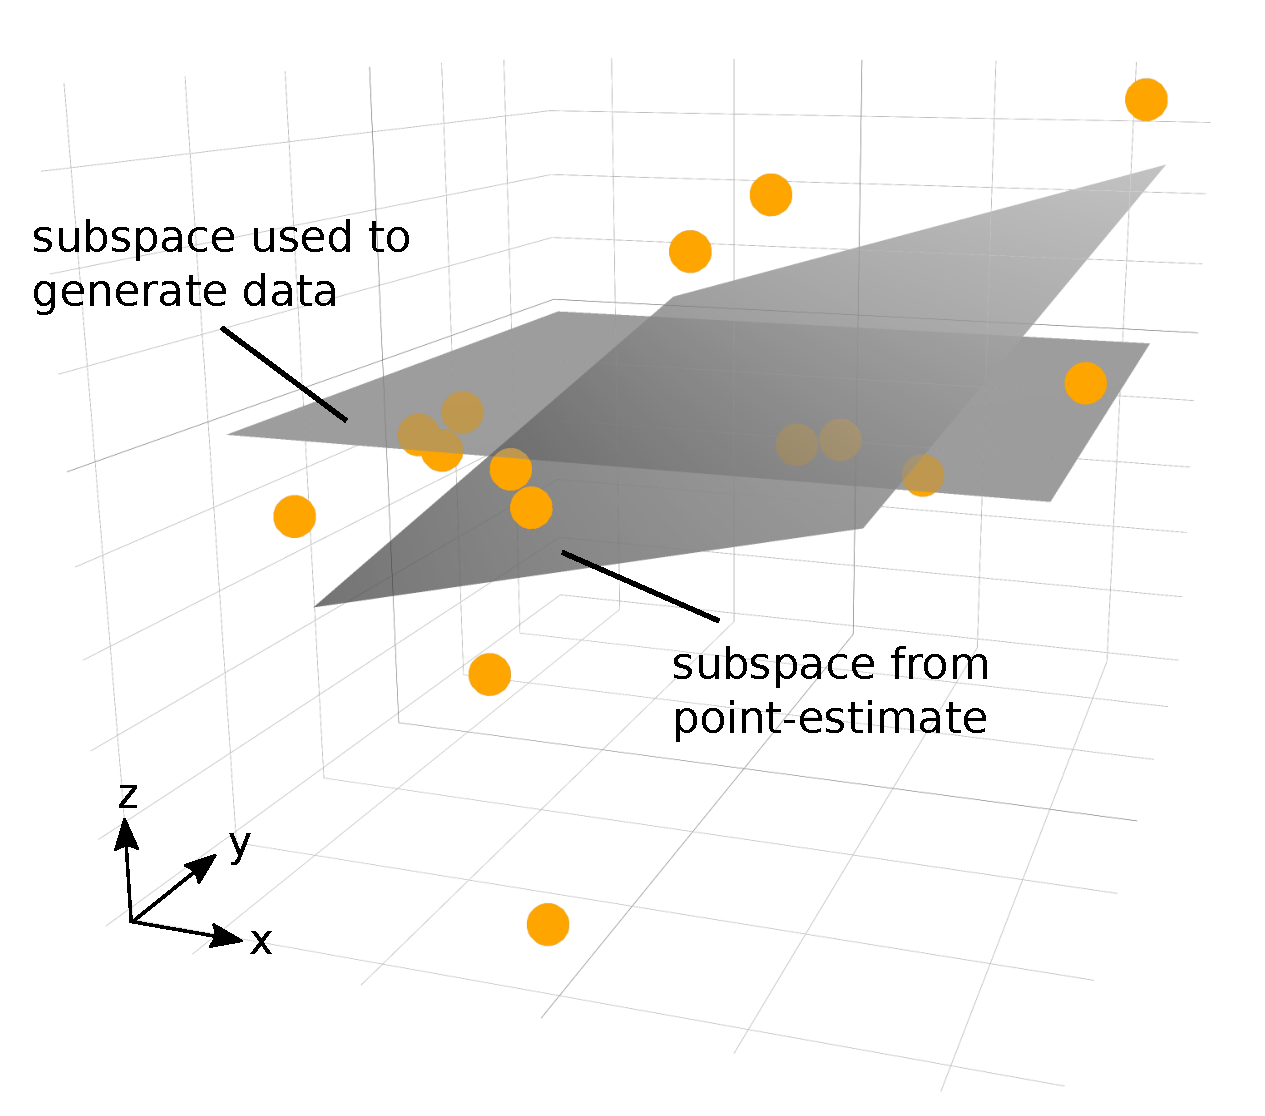
\includegraphics[width=0.5\textwidth]{figures/uncertainty_atz.pdf}
\vspace{.05in}
\caption{PCA finds a single orthogonal matrix in the Stiefel Manifold that is closest, in terms of average squared distance, to the set of points.  This point estimate can often mislead us from the true subspace, which in this case is the horizontal $(x,y)$-plane which was used to generate the noisy data. The data shown here is within the three-dimensional space parameterized by $x$, $y$, and $z$.  Alternatively, in Probabilistic PCA (PPCA) a posterior distribution is used to estimate the approximating subspace and also to quantify the uncertainty of the result.}
\label{fig:MleSubspaceEstimate}
\end{figure}

\noindent To ensure identifiability $W$ is constrained to be an orthogonal $n \times p$ matrix while $\Lambda$ is a diagonal matrix with positive, ordered elements. Because $\mb{x}_i$ is a linear transformation of a multivariate Gaussian, $\mb{z}_i$ can be integrated out of the model \ref{eq:PpcaGenerativeProcess} to yield the simplified model

\begin{eqnarray}
\label{eq:PpcaSimplifiedModel}
\mb{x}_i | W, \Lambda, \sigma^2 &\sim& \mathcal{N}_n(0, \textbf{C}).
\end{eqnarray}

\noindent where $\textbf{C} := W \Lambda^2 W^T + \sigma^2$ I \citep{murphy2012machine}. Letting $\hat{\Sigma} := (1/N) \sum_{i=1}^N \mb{x}_i \mb{x}_i^T$ denote the empirical covariance, matrix this gives us the simplified PPCA likelihood

\begin{eqnarray}
p(\mb{x}_1, \cdots, \mb{x}_N | W, \Lambda, \sigma^2) &=& -\frac{N}{2} \ln |\textbf{C}| - \frac{1}{2} \sum_{i=1}^N \mb{x}_i^T \textbf{C}^{-1} \mb{x}_i\\
&=& -\frac{N}{2} \ln |\textbf{C}| - \frac{N}{2} \mathrm{tr} (\textbf{C}^{-1} \hat{\Sigma}).
\label{eq:ppca_likelihood}
\end{eqnarray}

\noindent Traditional PCA corresponds to the closed-form maximum likelihood estimator for $W$ in the limit as $\sigma^2 \to 0$,  providing no measure of uncertainty for this point-estimate. Furthermore, for more elaborate models, the analytical form of the maximum-likelihood estimator is rarely known.

\noindent We used the Givens representation in Stan to infer the parameters in model \ref{eq:PpcaSimplifiedModel} from a simulated dataset with $n = 50$ and $p = 3$. For  $\Lambda$ and $\sigma^2$ we chose uniform priors over the positive real line and for $W$ we chose a uniform prior over the Stiefel manifold yielding the unnormalized posterior density

\begin{eqnarray}
p(W, \Lambda, \sigma^2 | \mb{x}_1, \cdots, \mb{x}_N) \propto p(\mb{x}_1, \cdots, \mb{x}_N | W, \Lambda, \sigma^2)
\end{eqnarray}

\noindent or in the Givens representation

\begin{eqnarray}
\label{eq:ppca_density_givens}
p(\Theta, \Lambda, \sigma^2 | \mb{x}_1, \cdots, \mb{x}_N) \propto p(\mb{x}_1, \cdots, \mb{x}_N | W(\Theta), \Lambda, \sigma^2)\, |J_{Y(\Theta)}(\Theta)|
\end{eqnarray}

\noindent where the latter term comes from Equation \ref{eq:final_change_of_measure}.

\noindent For the true value of the parameters we used the settings used by \citet{jauch2018random} in their experiments section: $\Lambda^2 = \mathrm{diag}(5, 3, 1.5)$, $\sigma^2 = 1$, and $W$ drawn uniformly from $V_{3, 50}$. For inference 10,000 samples were taken using Stan's NUTS algorithm with default settings. Table \ref{tab:ppca50} shows the posterior quantiles along with $\hat{R}$ and $n_{\mathrm{eff}}$ values for $\Lambda^2$ and $\sigma^2$. Like \citet{jauch2018random}, we plot histograms of the principal angle,

\begin{equation}
\phi_j = \mathrm{arccos}(E_j^T W_j),\, j=1,2,3
\end{equation}

\noindent between the columns, $W_j$, of posterior draws of $W$ and the columns of the first three eigenvectors of $\hat{\Sigma}$, $E_j$ (Figure \ref{fig:ppca50_principal_angle}).

\begin{table*}
\begin{tabular}{|c||ccccccc|}
\hline
Parameter & 2.5\% & 25\% & 50\% & 75\% & 97.5\% &  $\hat{R}$ & $n_{\mathrm{eff}}$\\
\hline
\hline
$\Lambda_1^2$  & 3.98 & 4.87 & 5.46 & 6.14 & 7.74 & 1.0 & 3,313\\
$\Lambda_2^2$  & 2.48 & 3.16 & 3.61 & 4.09 & 5.10 & 1.0 & 848\\
$\Lambda_2^2$  & 1.21 & 1.76 & 2.07 & 2.44 & 3.20 & 1.0 & 1,340 \\
$\sigma^2$ & 0.99 & 1.01 & 1.03 & 1.04 & 1.07 & 1.0 & 5,374\\
\hline
\end{tabular}
\caption{Posterior quantiles, $\hat{R}$, and $n_{\mathrm{eff}}$ values for $\Lambda^2$ and $\sigma^2$ computed over 10,000 posterior draws.}
\label{tab:ppca50}
\end{table*}

\begin{figure}[h]
\centering
\vspace{.1in}
\includegraphics[width=0.7\textwidth]{figures/jauche_sim_principal_angle.png}
\vspace{.05in}
\caption{Histograms of the principal angles between posterior samples of $W$ and the first three eigenvectors of $\hat{\Sigma}$.}
\label{fig:ppca50_principal_angle}
\end{figure}

\noindent Lastly, Figure \ref{fig:ppca50_coverage} shows the true values of $W$ used in the simulation along with the 80\% credible intervals, computed from posterior samples, of the marginal posterior distributions of the elements of $W$. 

\begin{figure}[h]
\centering
\vspace{.1in}
\includegraphics[width=0.9\textwidth]{figures/ppca50_coverage.png}
\vspace{.05in}
\caption{True values of $W$ used in the simulation along with 80\% credible intervals computed using draws of the posterior.}
\label{fig:ppca50_coverage}
\end{figure}


%%%%%%%%%%%%%%%%%%%%%%%%%
\subsection{Sparse PPCA}
%%%%%%%%%%%%%%%%%%%%%%%%%
To illustrate the utility of placing priors over the angle parameters, $\Theta$, of the Givens representation, we fit a PPCA model with sparse priors over $\Theta$ to simulated data generated from \ref{eq:PpcaGenerativeProcess}, with the same parameter settings as in the previous example, but with $W$ replaced with a sparse $50 \times 3$ matrix. Specifically, we drew $W$ uniformly from $V_{3,50}$, converted the result to the Givens representation, randomly set each angle to zero with probability 0.8, then converted the result back to the canonical representation. The result was an orthogonal $V_{3,50}$ matrix, $W$, with 85\% of its elements equal to zero.

\noindent For our model, we used the standard PPCA likelihood \ref{eq:ppca_likelihood} with uniform priors over $\Lambda^2$ and $\sigma^2$, but rather than placing a prior over $\Theta$ was uniform over the Stiefel manifold, we set $\Theta$ to follow the regularized horseshoe prior of \cite{piironen2017sparsity}, a commonly used sparsity-inducing prior. Formally, we set

\begin{eqnarray}
\theta_{ij} &\sim& \mathcal{N}(0, \tau^2 \tilde{\lambda}_{ij}^2),\; \tilde{\lambda}_{ij}^2 = \frac{c^2 \lambda_{ij}^2}{c^2 + \tau^2 \lambda_{ij}^2}\\
\lambda_{ij} &\sim& \mathrm{Half Cauchy}(0,1)\nonumber \\
\tau &\sim& \mathrm{Half Cauchy}(0,\tau_0)\nonumber \\
c^2 &\sim& \mathrm{Inverse Gamma}(\nu/2, \nu s^2/2)\nonumber
\end{eqnarray}

\noindent with hyper-parameters set to $\tau_0 = 0.01$, $\nu = 10$, and $s = \pi/4$ following the guidelines of \cite{piironen2017sparsity}. We took 10,000 posterior draws in Stan using the resulting unnormalized posterior density

\begin{eqnarray}
\label{eq:ppca_sparse_density_givens}
p(\Theta, \Lambda, \sigma^2 | \mb{x}_1, \cdots, \mb{x}_N) \propto p(\mb{x}_1, \cdots, \mb{x}_N | W(\Theta), \Lambda, \sigma^2)\, p(\Theta, \lambda, \tau, c^2).
\end{eqnarray}

\noindent Table \ref{tab:ppca50_sparse} shows a posterior summary for the sparse model versus the non-sparse corresponding to the density \ref{eq:ppca_density_givens}. While the marginal posterior distributions of $\Lambda^2$ and $\sigma^2$ are similar for both models, the sparse model expectedly results in a much sparser posterior distribution over $\Theta$ and thus $W$ (Figure \ref{fig:ppca50_coverage_sparse}). In particular for elements of $W$ that are truly zero, the marginal posterior distributions of the sparse model tend to concentrate much closer to zero, while for truly non-zero elements, the sparse model is able to concentrate posterior mass away from zero.

\begin{table*}
\begin{tabular}{|cc||ccccccc|}
\hline
Model & Parameter & 2.5\% & 25\% & 50\% & 75\% & 97.5\% &  $\hat{R}$ & $n_{\mathrm{eff}}$\\
\hline
\hline
Non-Sparse & $\Lambda_1^2$  & 3.69 & 4.48 & 4.95 & 5.52 & 6.88 & 1.0 & 3,938\\
Non-Sparse & $\Lambda_2^2$  & 2.66 & 3.38 & 3.80 & 4.25 & 5.16 & 1.0 & 1,828\\
Non-Sparse & $\Lambda_2^2$  & 0.18 & 0.94 & 1.27 & 1.62 & 2.39 & 1.0 & 366 \\
Non-Sparse &  $\sigma^2$ & 0.97 & 1.00 & 1.01 & 1.03 & 1.06 & 1.0 & 1,421\\
\hline
Sparse & $\Lambda_1^2$  & 3.71 & 4.48 & 4.97 & 5.58 & 6.91 & 1.0 & 5,425\\
Sparse & $\Lambda_2^2$  & 2.67 & 3.31 & 3.70 & 4.13 & 5.01 & 1.0 & 4,952\\
Sparse & $\Lambda_2^2$  & 0.78 & 1.15 & 1.38 & 1.63 & 2.24 & 1.0 & 4,779 \\
Sparse &  $\sigma^2$ & 0.97 & 1.00 & 1.01 & 1.03 & 1.05 & 1.0 & 7,191\\
\hline
\end{tabular}
\caption{$\hat{R}$ and $n_{\mathrm{eff}}$ values averaged over all elements of the matrix parameter $Y$. }
\label{tab:ppca50_sparse}
\end{table*}

\begin{figure}[h]
\centering
\vspace{.1in}
\includegraphics[width=0.99\textwidth]{figures/ppca50_coverage_sparse.png}
\vspace{.05in}
\caption{True values of $W$ used in the simulation along with 80\% posterior credible intervals computed using 10,000 draws of the posterior from the sparse and non-sparse models respectively. The posterior distribution of the sparse model places much more posterior mass closer to zero for values that are truly zero, while concentrating mass away from zero for truly non-zero values.}
\label{fig:ppca50_coverage_sparse}
\end{figure}

%%%%%%%%%%%%%%%%%%%%%%%%%
\subsection{The Network Eigenmodel}
%%%%%%%%%%%%%%%%%%%%%%%%%
To illustrate the Givens representation on a more elaborate model with orthogonal matrix parameters, we used it to infer the network eigenmodel of \cite{hoff2009simulation} on real data and compared it to EMHMC. The same model was inferred using EMHMC by \cite{byrne2013geodesic}. The data, which was originally described in \cite{butland2005interaction} and freely available in the R package \textit{eigenmodel}, consists of a symmetric $230 \times 230$ graph matrix, $Y$, which encodes whether the proteins in a protein network of size $n=230$ interact with one another.

\noindent The probability of a connection between all combinations of proteins can be described by the lower-triangular portion of a symmetric matrix of probabilities, however the network eigenmodel uses a much lower dimensional representation to represent this connectivity matrix. Specifically, given an orthogonal matrix $U$, a diagonal matrix $\Lambda$, and a scalar $c$, then letting $\Phi(\cdot)$ represent the probit link function, the model is described as follows:

\begin{eqnarray}
c &\sim& \mathcal{N}(0, 10^2)\\
\Lambda_i &\sim& \mathcal{N}(0, n),\, \forall i\\
Y_{ij} &\sim& \mathrm{Bernoulli} \left(\Phi ([U \Lambda U^T]_{ij} + c) \right),\, \forall i > j.
\end{eqnarray}

\noindent The Stan implementation using the Givens representation took approximately 300 seconds to collect 1000 samples, 500 of which were warmup. In contrast, EMHMC took 812 seconds to run the same 1000 samples using the hyperparameter values specified in  \cite{byrne2013geodesic}. Figure \ref{fig:eigennetwork_traceplots} compares traceplots for $c, \Lambda,$ and the elements of the top row $U$ for the 500 post warmup samples from each sampler. As mentioned in \cite{byrne2013geodesic} the non-ordering of the $\Lambda$ parameters results in a multimodality in the posterior whereby values of $\Lambda$ can be ``flipped". Computed $\hat{R}$ and $n_{\mathrm{eff}}$ for these parameters are shown in Table \ref{tab:rhat_neff_eigennetwork}.

\begin{figure}[h]
\centering
\vspace{.1in}
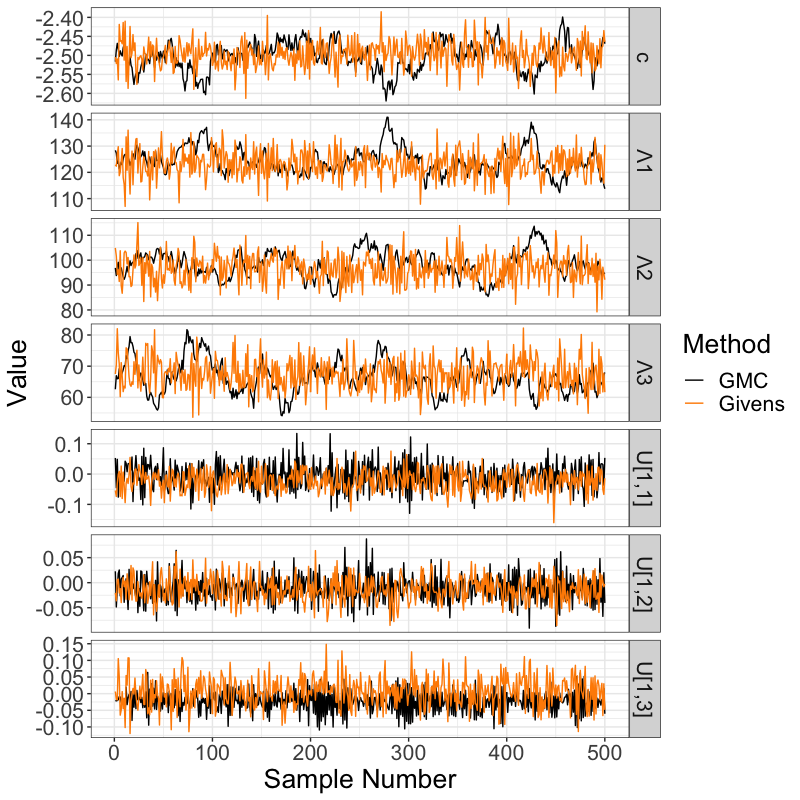
\includegraphics[width=0.8\textwidth]{figures/eigennetwork_traceplots.png}
\vspace{.05in}
\caption{Traceplots of samples from the Givens representation implementation in Stan and EMHMC reveal the multimodality in the elements of $\Lambda$. For brevity, only the top three elements of $U$ are shown.}
\label{fig:eigennetwork_traceplots}
\end{figure}

\begin{table*}
\begin{tabular}{|c||cc|cc|}
\hline
 & EMHMC & & Givens &\\
\hline
Parameter & $\hat{R}$ & $n_{\mathrm{eff}}$ & $\hat{R}$ & $n_{\mathrm{eff}}$\\
\hline
\hline
$c$ & 1.00 & 22 & 1.00 & 496\\
$\Lambda_1$ & 1.00 & 19 & 1.00 & 500\\
$\Lambda_2$ & 1.00 & 23 & 1.00 & 500\\
$\Lambda_3$ & 1.10 & 18 & 1.00 & 500\\
$U[1,1]$ & 1.01 & 500 & 1.00 & 500\\
$U[2,1]$ & 1.00 & 500 & 1.00 & 500\\
$U[3,1]$ & 1.02 & 500 & 1.00 & 500\\
\hline
\end{tabular}
\caption{$\hat{R}$ and $n_{\mathrm{eff}}$ values for the parameters in the network eigenmodel. For brevity, only three of the matrix parameters are shown.}
\label{tab:rhat_neff_eigennetwork}
\end{table*}

%%%%%%%%%%%%%%%%%%%%%%%%%
%%%%%%%%%%%%%%%%%%%%%%%%%
%%%%%%%%%%%%%%%%%%%%%%%%%
\section{Discussion}\label{discussion}
%%%%%%%%%%%%%%%%%%%%%%%%%
%%%%%%%%%%%%%%%%%%%%%%%%%
%%%%%%%%%%%%%%%%%%%%%%%%%
We have introduced a systematic approach to incorporating the Givens representation into a general Bayesian inference framework for the purpose of inferring general Bayesian models with orthogonal matrix parameters. Our approach overcomes practical barriers to using the Givens representation in such a setting including having to efficiently compute the measure adjustment term and dealing with singularities caused by differences in topology. Furthermore, we also provided an intuitive explanation behind the Givens representation that is accessible to statisticians and followed with practical examples for which we provide code. We expect our approach can be used quite widely in practice by a variety of practitioners.

%%%%%%%%%%%%%%%%%%%%%%%%%
%%%%%%%%%%%%%%%%%%%%%%%%%
%%%%%%%%%%%%%%%%%%%%%%%%%
\appendix
\section{Deriving the Change of Measure Term}
%%%%%%%%%%%%%%%%%%%%%%%%%
%%%%%%%%%%%%%%%%%%%%%%%%%
%%%%%%%%%%%%%%%%%%%%%%%%%
We derive the simplified form (Expression \ref{eq:final_change_of_measure}) of the differential form (Expression \ref{eq:WedgeForm}). We point out that \cite{khatri1977mises} provide a similar expression for a slightly different representation, but do not offer a derivation.

\noindent We start with the determinant of the matrix form of the change of measure term from Expression \ref{eq:measure_matrix_form} (reproduced below):

\begin{equation}
\begin{pmatrix}
G_{2:n}^T J_{Y_1(\Theta)}(\Theta)\\
G_{3:n}^T J_{Y_2(\Theta)}(\Theta)\\
\vdots\\
G_{p:n}^T J_{Y_p(\Theta)}(\Theta)
\end{pmatrix}
\end{equation}

\noindent For $l = 1, \cdots, n$, let us define the following shorthand notation

\begin{equation}
\partial_{i,i+l} Y_k := \frac{\partial}{\partial \theta_{i,i+l}} Y_k
\end{equation}

\noindent and

\begin{equation}
\partial_{i} Y_k
:=
\begin{pmatrix}
\partial_{i,i+1} Y_k & \partial_{i,i+2} Y_k & \cdots & \partial_{in} Y_k.
\end{pmatrix}
\end{equation}

\noindent In the new notation Equation can be written in the following block matrix form:

\begin{equation}
\label{eq:matrix_blockform}
\begin{pmatrix}
G_{2:n}^T \partial_{1} Y_1 &G_{2:n}^T \partial_{2} Y_1 & \cdots & G_{2:n}^T \partial_{p} Y_1\\
G_{3:n}^T \partial_{1} Y_2 &G_{3:n}^T \partial_{2} Y_2 & \cdots & G_{3:n}^T \partial_{p} Y_2\\
\vdots & \vdots & \ddots & \vdots\\
G_{p:n}^T \partial_{1} Y_p &G_{p:n}^T \partial_{2} Y_p & \cdots & G_{p:n}^T \partial_{p} Y_p\\
\end{pmatrix}.
\end{equation}

\noindent First note that the block matrices above the diagonal are all zero.  This can be seen by noting that the rotations in the Givens representation involving elements greater than $i$ will not affect $e_i$, i.e. letting $R_i := R_{i,i+1} \cdots R_{in}$,

\begin{eqnarray}
Y_i = R_1 R_2 \cdots R_p e_i = R_1 \cdots R_i e_i.
\end{eqnarray}

\noindent Thus for $j > i$, $\partial_j Y_i = 0$ and the determinant of Expression \ref{eq:matrix_blockform} simplifies to the product of the determinant of the matrices on the diagonal i.e. the following expression:

\begin{equation}
\label{eq:det_of_blocks}
\prod_{i=1}^p \det \left( G_{i+1:n}^T \partial_{i} Y_i \right).
\end{equation}

%%%%%%%%%%%%%%%%%%%%%%%%%
\subsection{Simplifying Diagonal Block Terms}
%%%%%%%%%%%%%%%%%%%%%%%%%
Let $I_{i}$ denote the first $i$ columns of the $n \times n$ identity matrix and let $I_{-i}$ represent the last $n-i$ columns. The term $G_{i+1:n}^T$ in Expression \ref{eq:det_of_blocks} can be written as

\begin{equation}
G_{i+1:n}^T = I_{-i}^T G^T = I_{-i}^T R_p^T \cdots R_1^T.
\end{equation}

\noindent To simplify the diagonal block determinant terms in Expression \ref{eq:det_of_blocks} we take advantage of the following fact

\begin{eqnarray}
\det \left( G_{i+1:n}^T \partial_i Y_i  \right)  &=& \det \left( I_{-i}^T R_p^T \cdots R_1^T \right) =  \det\left( I_{-i}^T R_i^T \cdots R_1^T \partial_i Y_i \right).
\end{eqnarray}

\noindent In other words, the terms $R_p^T \cdots R_{i+1}^T$ have no effect on the determinant. This can by first separating terms so that

\begin{eqnarray}
\det\left(G_{i+1:n}^T \partial_{i} Y_i \right) &=& \det\left( \underbrace{I_{-i}^T}_{(n-i) \times n} R_p^T \cdots R_1^T \underbrace{\partial_i Y_i}_{n \times (n-i)} \right)\\
&=& \det\left(
I_{-i}^T
\left[ R_p^T \cdots R_{i+1}^T\right] \left[ R_i^T \cdots R_1^T \partial_i Y_i \right] \right)
\end{eqnarray}

\noindent then noticing that $R_{i+1} \cdots R_p$ only effects the first $i$ columns of the identity matrix so 

\begin{eqnarray}
I_{-i}^T
\left[ R_p^T \cdots R_{i+1}^T\right]  &=& \left( R_{i+1} \cdots R_p\, I_{-i} \right)^T = \left( I_{-i} \right)^T.
\end{eqnarray}

\noindent Thus Expression \ref{eq:det_of_blocks} is equivalent to

\begin{equation}
\label{eq:simplified_determinant}
\prod_{i=1}^p \det \left( I_{-i}^T R_i^T \cdots R_1^T \partial_{i} Y_i \right).
\end{equation}

\noindent Now consider the $k,l$ element of the $(n-i) \times (n-i)$ block matrix $I_{-i}^T R_i^T \cdots R_1^T \partial_{i} Y_i $. This can be written as 

\begin{eqnarray}
\label{eq:kl_element}
e_{i+k}^T R_i^T \cdots R_1^T \partial_{i,i+l} Y_i &=&  e_{i+k}^T R_i^T \cdots R_1^T \partial_{i,i+l} (R_1 \cdots R_i e_i)\nonumber \\ \nonumber
&=&  e_{i+k}^T R_i^T \cdots R_1^T R_1 \cdots R_{i-1} (\partial_{i,i+l} R_i e_i)\nonumber \\ 
&=&  e_{i+k}^T R_i^T  (\partial_{i,i+l} R_i e_i).
\end{eqnarray}

\noindent Since  $e_{i+k}^T R_i^T R_i e_i =0$, taking the derivatives of both sides gives and applying the product rule yields

\begin{eqnarray}
&&\partial_{i,i+l} (e_{i+k}^T R_i^T R_i e_i) = \partial_{i,i+l} 0\nonumber \\
&\Rightarrow& (\partial_{i,i+l} e_{i+k}^T R_i^T) R_i e_i + e_{i+k}^T R_i^T ( \partial_{i,i+l}R_i e_i) = 0\nonumber \\
&\Rightarrow& e_{i+k}^T R_i^T  (\partial_{i,i+l}R_i e_i) = -(\partial_{i,i+l} e_{i+k}^T R_i^T) R_i e_i.
\end{eqnarray}

\noindent Combining this fact with Expression \ref{eq:kl_element}, the expression for the $k,l$ element of $I_{-i}^T R_i^T \cdots R_1^T \partial_{i} Y_i $ becomes $-(\partial_{i,i+l} e_{i+k}^T R_i^T) R_i e_i$.

\noindent However, note that

\begin{eqnarray}
e_{i+k}^T R_i^T &=&  e_{i+k}^T R_{in}^T \cdots R_{i,i+1}^T = e_{i+k}^T R_{i,i+k}^T \cdots R_{i,i+1}^T,
\end{eqnarray}

\noindent and the partial derivative of this expression with respect to $i,i+l$ is zero when $k > l$. Thus it is apparent that $I_{-i}^T R_i^T \cdots R_1^T \partial_{i} Y_i $ contains zeros above the diagonal and that $\det \left( I_{-i}^T R_i^T \cdots R_1^T \partial_{i} Y_i \right)$ is simply the product of the diagonal elements of the matrix.

%%%%%%%%%%%%%%%%%%%%%%%%%
\subsection{Diagonal Elements of the Block Matrices}
%%%%%%%%%%%%%%%%%%%%%%%%%
To obtain the diagonal terms of the block matrices we directly compute $-\partial_{i,i+l} e_{i+k}^T R_i^T$ for $l=k$, $R_i e_i$, and their inner-product. Defining $D_{ij} := \partial_{ij} R_{ij}$,

\begin{eqnarray}
-\partial_{i,i+k} R_i e_{i+k} &=&   -\partial_{i,i+k} (R_{i,i+1} \cdots R_{i,i+k} e_{i+k}) \\
&=& -R_{i,i+1} \cdots R_{i,i+k-1} D_{i,i+k} e_{i+k} \\
\\
&=&
R_{i,i+1} \cdots R_{i,i+k-1}
\begin{pmatrix}
0\\
\vdots\\
0\\
\cos \theta_{i,i+k}\\
0\\
\vdots\\
0\\
\sin \theta_{i,i+k}\\
0\\
\vdots\\
0
\end{pmatrix}
\\
&=&
R_{i,i+1} \cdots R_{i,i+k-2}
\begin{pmatrix}
0\\
\vdots\\
0\\
\cos \theta_{i,i+k-1} \cos \theta_{i,i+k}\\
0\\
\vdots\\
0\\
\sin \theta_{i,i+k-1} \cos \theta_{i,i+k}\\
\sin \theta_{i,i+k}\\
0\\
\vdots\\
0
\end{pmatrix}
\\
&=&
\begin{pmatrix}
0\\
\vdots\\
0\\
\cos \theta_{i,i+1} \cos \theta_{i,i+2} \cdots \cos \theta_{i,i+k-1} \cos \theta_{i,i+k}\\
\sin \theta_{i,i+1} \cos \theta_{i,i+2} \cdots \cos \theta_{i,i+k-1} \cos \theta_{i,i+k}\\
\vdots\\
\sin \theta_{i,i+k-1} \cos \theta_{i,i+k}\\
\sin \theta_{i,i+k}\\
0\\
\vdots\\
0
\end{pmatrix}
\\
\end{eqnarray}

\noindent which is zero up to the $i$th spot and after the $i+k$th spot.

\begin{eqnarray}
R_i e_i &=&   R_{i,i+1} \cdots R_{in} e_i \\
\\
&=&
\begin{pmatrix}
0\\
\vdots\\
0\\
\cos \theta_{i,i+1} \cos \theta_{i,i+2} \cdots \cos \theta_{i,n-1} \cos \theta_{in}\\
\sin \theta_{i,i+1} \cos \theta_{i,i+2} \cdots \cos \theta_{i,n-1} \cos \theta_{in}\\
\vdots\\
\sin \theta_{i,n-1} \cos \theta_{in}\\
\sin \theta_{in}
\end{pmatrix}.
\end{eqnarray}

\noindent Finally, directly computing the inner-product of $-\partial_{i,i+l} e_{i+k}^T R_i^T$ and $R_i e_i$:

\begin{eqnarray}
-(\partial_{i,i+l} e_{i+k}^T R_i^T) (R_i e_i)
&=&
\cos^2 \theta_{i,i+1} \cos^2 \theta_{i,i+2}  \cdots \cos^2 \theta_{i,i+k}  \cos \theta_{i,i+k+1} \cdots \cos \theta_{in} \nonumber\\
&+& \sin^2 \theta_{i,i+1} \cos^2 \theta_{i,i+2} \cdots \cos^2 \theta_{i,i+k}  \cos \theta_{i,i+k+1} \cdots \cos \theta_{in} \nonumber\\
&+&  \sin^2 \theta_{i,i+2} \cos^2 \theta_{i,i+3} \cdots \cos^2 \theta_{i,i+k}  \cos \theta_{i,i+k+1} \cdots \cos \theta_{in} \nonumber\\
&\vdots&  \nonumber\\
&+&  \sin^2 \theta_{i,i+k} \cos \theta_{i,i+k+1} \cdots \cos \theta_{in}
 \nonumber\\
&=&
\cos^2 \theta_{i,i+2} \cos^2 \theta_{i,i+3}  \cdots \cos^2 \theta_{i,i+k}  \cos \theta_{i,i+k+1} \cdots \cos \theta_{in}  \nonumber\\
&+&  \sin^2 \theta_{i,i+2} \cos^2 \theta_{i,i+3} \cdots \cos^2 \theta_{i,i+k}  \cos \theta_{i,i+k+1} \cdots \cos \theta_{in}  \nonumber\\
&\vdots&  \nonumber\\
&+&  \sin^2 \theta_{i,i+k} \cos \theta_{i,i+k+1} \cdots \cos \theta_{in}  \nonumber\\
&=& \cdots \nonumber\\
&=& \cos \theta_{i,i+k+1} \cdots \cos \theta_{in}\nonumber\\
&=& \prod_{k=i+1}^n \cos \theta_{ik}.
\end{eqnarray}

\noindent Thus the determinant of the entire block matrix $I_{-i}^T R_i^T \cdots R_1^T \partial_{i} Y_i $ simplifies to

\begin{equation}
\prod_{k=i+1}^n \left( \prod_{j=k+1}^n \cos \theta_{ik} \right) = \prod_{j=i+1}^n \cos^{j-i-1} \theta_{ij}.
\end{equation}

\noindent Combining this with Expression \ref{eq:simplified_determinant} yields finally

\begin{eqnarray}
\prod_{i=1}^p \det \left( I_{-i}^T R_i^T \cdots R_1^T \partial_{i} Y_i \right) = \prod_{i=1}^p \prod_{j=i+1}^n \cos^{j-i-1} \theta_{ij}.
\end{eqnarray}

%%%%%%%%%%%%%%%%%%%%%%%%%
%%%%%%%%%%%%%%%%%%%%%%%%%
%%%%%%%%%%%%%%%%%%%%%%%%%
\bibliographystyle{ba}
\bibliography{sample}

%\begin{acknowledgement}
Research reported in this publication was performed by the Systems Biology Coagulopathy of Trauma Program of the US Army Medical Research and Materiel Command under award number W911QY-15-C-0026. The author P.J.A acknowledges support from research grant DOE ASCR CM4 DE-SC0009254 and NSF DMS - 1616353.
%\end{acknowledgement}

\end{document}

